% Requires some preamble before using such as:
% This appendix describes in full detail the two functional forms
% most widely used in CGE models-the constant-elasticity-of-substitution
% (CES) and constant-elasticity-of-transformation (CET) functions.
CES functions are widely used in demand functions where substitutability
across different products and/or factors is needed and where the main objective
is to minimize cost. CET functions are broadly used to determine supply
functions across different markets where the main objective is to maximize
revenues. The two are very similar in many ways and the algebraic derivations
below will be more detailed for the CES function.

\section{The CES function}
\subsection{Basic formulas}

In production, the CES function is used to select an optimal combination of
inputs (either goods and/or factors) subject to a CES production function.
In consumer demand, the CES is used as a utility (or sub-utility) or preference function.
In either case, the purpose is to minimize the cost of purchasing the 'inputs'
subject to the production or utility function. In generic terms the system
takes the following form:

\begin{displaymath}
\min_{X_i}{\sum\limits_{i}{{{P}_{i}}{{X}_{i}}}}
\end{displaymath}

\noindent subject to the constraint:

\begin{displaymath}
V=A{{\left[ \sum\limits_{i}{{{a}_{i}}{{({{\lambda }_{i}}{{X}_{i}})}^{\rho }}} \right]}^{1/\rho }}
\end{displaymath}

The objective function represents aggregate expenditure. The constraint expression will be referred
to as the CES primal function. The parameter $A$ is an aggregate shifter that can be used to shift
the overall production function (or utility function). Each input, $X_i$, is multiplied by an
input-specific shifter, $\lambda_i$, that can be used to implement input-specific productivity
increases (for example biased technological change), or specific changes in consumer preferences.
The (primal) share coefficients, $a_i$, are typically calibrated to some base year data and held
fixed. The CES exponent, $\rho$, is linked to the curvature of the CES function (and will be
explained further below). For given component prices, $P_i$, and a given level of production or
utility $V$, solving the optimization program above will yield optimal demand functions for the
inputs, $X_i$.

The Lagrangian can be set up as:

\begin{displaymath}
\mathcal{L}=\sum\limits_{i}{{{P}_{i}}{{X}_{i}}}+\Lambda \left( V-A{{\left[
\sum\limits_{i}{{{a}_{i}}{{({{\lambda }_{i}}{{X}_{i}})}^{\rho }}} \right]}^{1/\rho }} \right)
\end{displaymath}

Taking the partial derivative with respect to $X_i$ and the Lagrange multiplier $\Lambda$ yields the
following system of equations:

\begin{displaymath}
{{P}_{i}}=\Lambda {{a}_{i}}\lambda _{i}^{\rho }X_{i}^{\rho -1}A{{\left[ \sum\limits_{i}{{{a}_{i}}
{{({{\lambda }_{i}}{{X}_{i}})}^{\rho }}}
\right]}^{(1-\rho )/\rho }}=\Lambda {{a}_{i}}{{A}^{\rho }}
\lambda_{i}^{\rho }X_{i}^{\rho -1}{{V}^{1-\rho }}
\end{displaymath}

\begin{displaymath}
V=A{{\left[ \sum\limits_{i}{{{a}_{i}}{{({{\Lambda }_{i}}{{X}_{i}})}^{\rho }}} \right]}^{1/\rho }}
\end{displaymath}

Taking the first expression, it can be multiplied by $X_i$, and then summed. This of course is
equal to the value of the bundle, i.e. $P.V$, where $P$ is the aggregate price:

\begin{displaymath}
P.V=\sum\limits_{i}{{{P}_{i}}{{X}_{i}}}=\Lambda {{V}^{1-\rho }}{{A}^{\rho }}
\sum\limits_{i}{{{a}_{i}}\lambda_{i}^{\rho }X_{i}^{\rho }}=
\Lambda {{V}^{1-\rho }}{{V}^{\rho }}=\Lambda V
\end{displaymath}

This shows that $\Lambda$, the Lagrange multiplier is the same as the aggregate price, $P$. We can
re-arrange expression above to get an expression for optimal input demand, where $\Lambda$ is
replaced by $P$:

\begin{displaymath}
{{X}_{i}}=a_{i}^{1/(1-\rho )}{{A}^{\rho /(1-\rho )}}{{\left( \frac{P}{{{P}_{i}}}
\right)}^{1/(1-\rho )}}\lambda_{i}^{\rho /(1-\rho )}V
\end{displaymath}

We finally end up with the following expression, where the CES primal exponent, $\rho$, is
replaced by the so-called CES elasticity of substitution, $\sigma$:

\begin{equation} \label{eq:CESFOC}
{{X}_{i}}={{\alpha }_{i}} {{\left( A \lambda _{i} \right) }^{\sigma -1}}
{{\left( \frac{P}{{{P}_{i}}} \right)}^{\sigma }} V
\end{equation}

\noindent where we made the following substitutions:

\begin{displaymath}
\sigma =\frac{1}{1-\rho }\Leftrightarrow \rho =\frac{\sigma -1}{\sigma }
\Leftrightarrow \frac{\rho }{1-\rho }=\sigma -1\Leftrightarrow \rho .\sigma =\sigma -1
\end{displaymath}

\noindent and
\begin{displaymath}
{{\alpha }_{i}}=a_{i}^{1/(1-\rho )}=a_{i}^{\sigma }\Leftrightarrow {{a}_{i}}=\alpha _{i}^{1/\sigma }
\end{displaymath}

Abstracting from the technology parameters, the demand equation implies that demand for
'input' $X_i$ is a (volume) share of total demand $V$. The share, with equal prices is simply
equal to $\alpha_i$. With a positive elasticity of substitution, the share is sensitive to the
ratio of prices relative to the aggregate price index. Since the component price is in the
denominator, the demand for that component declines if its price rises relative to the average
and vice versa if its price declines vis-\`a-vis the average price. The $\alpha$ parameters will be
referred to as the CES dual share parameters (for reasons described below), and the $a$ parameters
are the primal CES share parameters. Notice that expression (\ref{eq:CESFOC}) simplifies if it is
expressed in terms of efficiency inputs, $X^e$ and efficiency prices, $P^e$:

\begin{displaymath}
X_{i}^{e}={{\alpha }_{i}}{{A}^{\sigma -1}}{{\left( \frac{P}{P_{i}^{e}} \right)}^{\sigma }}V
\end{displaymath}

\noindent where

\begin{displaymath}
X_{i}^{e}={{\lambda }_{i}}{{X}_{i}}\
\end{displaymath}

\noindent and

\begin{displaymath}
P_{i}^{e}=\frac{{{P}_{i}}}{{{\lambda }_{i}}}\
\end{displaymath}

The aggregate price $P$ can be determined using two expressions. The first is the zero profit
condition:

\begin{displaymath}
P=\frac{\sum\limits_{i}{{{P}_{i}}{{X}_{i}}}}{V}
\end{displaymath}

The other is by inserting the optimal demand relation $X_i$ (equation~\ref{eq:CESFOC})
in the zero profit condition :

\begin{displaymath}
P.V=\sum\limits_{i}{{{P}_{i}}{{X}_{i}}}={{A}^{\sigma -1}}{{\sum\limits_{i}{{{P}_{i}}
{{\alpha }_{i}}\left( \frac{P}{{{P}_{i}}} \right)}}^{\sigma }}\lambda _{i}^{\sigma -1}V={{P}^{\sigma }}{{A}^{\sigma -1}}V{{\sum\limits_{i}{{{\alpha }_{i}}\left( \frac{{{P}_{i}}}{{{\lambda }_{i}}} \right)}}^{1-\sigma }}
\end{displaymath}

The $V$'s cancel out, and the aggregate price can then be expressed by the following formula:

\begin{equation} \label{eq:CESDual}
P=\frac{1}{A}{{\left[ {{\sum\limits_{i}{{{\alpha }_{i}}\left( \frac{{{P}_{i}}}{{{\lambda }_{i}}}
\right)}}^{1-\sigma }} \right]}^{1/(1-\sigma )}}
= \frac{1}{A}{{\left[ {{\sum\limits_{i}{{{\alpha }_{i}}\left( P_{i}^{e} \right)}}^{1-\sigma }}
\right]}^{1/(1-\sigma )}}
\end{equation}

This is sometimes referred to as the dual price expression. It has virtually the same functional
form as the CES primal, which is a CES aggregation of the input volumes using the primal share
parameters as weights. The CES dual price formula is a CES aggregation of the input prices using
the CES dual share parameters as weights and a different exponent. In a CGE model, the zero-profit
condition or the dual price formula can be used interchangeably (with the proviso that the
substitution elasticity differs from~1).\footnote{We shall see below that when the substitution
elasticity is 1, both primal and dual expressions take a different functional form.}
There is a simple formula for the budget shares given by:

\begin{equation} \label{eq:CESShare}
{{s}_{i}}=\frac{{{P}_{i}}{{X}_{i}}}{P.V}={{\alpha }_{i}}
{{\left(A{\lambda _{i}} \right)}^{\sigma -1}}
{{\left( \frac{P}{{{P}_{i}}} \right)}^{\sigma }}V\left( \frac{{{P}_{i}}}{P}
\right)\frac{1}{V}={{\alpha }_{i}}{{\left(A{\lambda _{i}} \right)}^{\sigma -1}}
{{\left( \frac{P}{{{P}_{i}}} \right)}^{\sigma -1}}
\end{equation}

Notice that this expression for the budget shares is only a function of prices. With the technology
parameters set to 1, this simplifies further to:

\begin{displaymath}
{{s}_{i}}={{\alpha }_{i}}{{\left( \frac{P}{{{P}_{i}}} \right)}^{\sigma -1}}
\end{displaymath}

It turns out that the parameter $\sigma$ measures the elasticity of substitution for the CES
function and is constant over the entire domain. The elasticity of substitution is an indication of
the curvature of an isoquant, see \cite{Varian1992}, i.e. it measures the rate of change of the ratio of
inputs (in a 2-input case), relative to the change in their relative prices. For example, if the CES
combines capital and labor to form output, a large substitution elasticity suggests that the
factor proportions will change rapidly as one of the inputs becomes cheaper relative to the
other. There are two limiting cases of interest. If the substitution elasticity is zero,
then there is no substitution across inputs and the optimal choice is to use them in fixed
proportion. At the other extreme, if the substitution elasticity is infinite, this is equivalent
to saying the inputs are identical, and in this case, in equilibrium, the two inputs would have
the same price. This could potentially be the case for electricity production. If there is a
regional or national buyer of electricity, the buyer is most likely indifferent about how the
electricity is produced and thus will purchase from the lowest cost producer (a perhaps
somewhat simplified view of electricity markets.) This implies that the cost of the electricity
inputs, from all sources (e.g. thermal, nuclear, etc.) would be (nearly) identical.

The elasticity of substitution across inputs is defined by the following formula:

\begin{displaymath}
\sigma =\frac{\partial \left( \frac{{{X}_{i}}}{{{X}_{j}}} \right)}{\partial \left(
\frac{{{P}_{i}}}{{{P}_{j}}} \right)}\frac{\left( \frac{{{P}_{i}}}{{{P}_{j}}}
\right)}{\left( \frac{{{X}_{i}}}{{{X}_{j}}} \right)}
\end{displaymath}

The ratio of the optimal inputs using expression (\ref{eq:CESFOC}) is:

\begin{displaymath}
\frac{{{\alpha }_{i}}}{{{\alpha }_{j}}}{{\left( \frac{{{P}_{i}}}{{{P}_{j}}} \right)}^{-
\sigma }}{{\left( \frac{{{\lambda }_{i}}}{{{\lambda }_{j}}} \right)}^{\sigma -1}}
\end{displaymath}

Taking the partial derivative of the expression with respect to the ratio $P_i/P_j$ and
multiplying it by the second term of the elasticity of substitution yields the conclusion that the
substitution elasticity is $-\sigma$. It is logical that it is negative. If the price of one input
increases, say labor, relative to the other, say capital, producers would substitute away from labor
towards capital, i.e. the ratio of labor to capital would drop as the price of labor increases
relative to capital. \cite{Varian1992} in fact defines the elasticity of substitution in terms of
the absolute value of the technical rate of substitution, that measures the slope of the budget
line. Numerically what it represents is the relative change in the ratios. If $\sigma$ is 1,
for example, and the price of labor increases by 10 percent relative to capital, the labor to
capital ratio would decrease by (around) 10 percent.\footnote{The elasticity is a marginal concept
that holds only approximately for large changes.} The higher is $\sigma$, the more the
proportion changes.

\subsection{Special cases}

There are three special cases that require additional derivations due to numerical restrictions
on the primal and dual exponents. A substitution elasticity of 0 is clearly a special case and
is referred to as a Leontief technology. From the dual price formula, it is clear that $\sigma$
equal to~1 is a special case and is known as a Cobb-Douglas technology (or utility function).
Finally, a value of $\rho$ equal to 1 corresponds to infinite substitution elasticity and a
linear primal aggregation function. This is also referred to as a case of perfect substitution.

\subsubsection{The Leontief case}

The first special case is for the so-called Leontief functional form.\footnote{Leontief, winner of
the 1973 Nobel prize in Economics, is renowned for his work on input-output tables, much of which
focused on fixed input technologies (!!!! reference).}  In this case the substitution elasticity
is~0 and corresponds to a value for $\rho$ that is ${-\infty}$. In this case the optimization
program takes the following form:\footnote{!!!! need a reference}

\begin{displaymath}
\min_{X_i}{\sum\limits_i{P_iX_i}}
\end{displaymath}

\noindent subject to the constraint:

\begin{displaymath}
V=\min \left( \frac{{{a}_{i}}}{{{\lambda }_{i}}{{X}_{i}}} \right)
\end{displaymath}

The visual implementation has L-shaped isoquants. The Leontief technology constraint or
production/utility function is discontinuous. Fortunately, the optimal demand functions are easy to
implement and are just special cases of expression (\ref{eq:CESFOC}):

\begin{displaymath}
{{X}_{i}}=\frac{{{\alpha }_{i}}}{{{\lambda }_{i}}}\frac{V}{A}
\end{displaymath}

\begin{displaymath}
P=\frac{1}{A}\sum\limits_{i}{{{\alpha }_{i}}\left( \frac{{{P}_{i}}}{{{\lambda }_{i}}}
\right)}
\end{displaymath}

Thus the Leontief specification implies that inputs are always in fixed proportion relative to
output and the aggregate price is simply the linear weighted aggregation of the input prices, where
the weights are given by the input-output coefficients, adjusted by changes in efficiency. The
efficiency parameter has a nice intuitive interpretation in this case. Say $\lambda$ increases
by~10 percent, then demand for the input declines by 10 percent.

\subsubsection{The Cobb-Douglas function}

Another special case is the so-called Cobb-Douglas function, very frequently used in
introductory text books in microeconomics. The Cobb-Douglas function has a substitution
elasticity of 1 implying that $\rho$ is equal to 0. Clearly, this creates a problem for specifying
the CES primal function as well as the CES dual price function. As with the Leontief, the optimal
demand conditions are given by expression (\ref{eq:CESFOC}), with $\sigma$ set to 1:

\begin{displaymath}
{{X}_{i}}={{\alpha }_{i}}\left( \frac{P}{{{P}_{i}}} \right)V\Leftrightarrow s{{
}_{i}}=\frac{{{P}_{i}}{{X}_{i}}}{P.V}={{\alpha }_{i}}
\end{displaymath}

The Cobb-Douglas specification has constant budget shares irrespective of relative prices
(and changes in technology). Another implication of the Cobb-Douglas specification is that the
dual shares must add up to~1 as they are equivalent to the budget shares. By definition, as well,
the primal and dual shares are the same. The Cobb-Douglas primal and dual price functions have the
following expressions:

\begin{displaymath}
V=A{{\prod\limits_{i}{\left( {{\lambda }_{i}}{{X}_{i}} \right)}}^{{{\alpha }_{i}}}}
\end{displaymath}

\begin{displaymath}
P=\frac{1}{A}{{\prod\limits_{i}{\left( \frac{{{P}_{i}}}{{{\alpha }_{i}}{{\lambda
}_{i}}} \right)}}^{{{\alpha }_{i}}}}
\end{displaymath}

Rather than code the Cobb-Douglas function as a special case, many modelers choose to
replace the elasticity of~1 with a value close to~1 such as~1.01. This would have only marginal
repercussions on the results.

\subsubsection{Perfect substitution}

The third special case is for a substitution elasticity of infinity. In this case $\rho$ takes the
value of~1 and the primal function is a straight linear aggregation of the inputs. The optimal
demand conditions cannot be used in the case of an infinite substitution elasticity. In its stead,
the optimal demand condition is replaced with the law-of-one-price, adjusted by efficiency
differentials, and the zero profit condition is replaced with the CES primal function, i.e. the
linear weighted aggregation of the inputs:

\begin{displaymath}
\frac{{{P}_{i}}}{{{\alpha }_{i}}{{\lambda }_{i}}}=P
\end{displaymath}

\begin{displaymath}
V=\sum\limits_{i}{{{\alpha }_{i}}{{\lambda }_{i}}{{X}_{i}}}
\end{displaymath}

The aggregation function can be replaced by the zero profit condition:\footnote{Modelers have
the choice of using the primal aggregation function or the revenue
function. The latter holds in all three special cases for the substitution elasticity.}

\begin{displaymath}
P.V=\sum\limits_{i}{{{P}_{i}}{{X}_{i}}}
\end{displaymath}

\subsection{Calibration of the CES function}

\ifCESDetail
\subsubsection{Standard calibration}
\fi

Calibration typically involves inverting functional forms to evaluate the value of a parameter
given initial values for variables. Prices and volumes, $P_i$, $X_i$, $V$ and $P$, are
normally initialized to a given database or SAM. This may or may not include actual
price/volume splits. If not, prices will typically be initialized at unit value---potentially
adjusted for a price wedge such as a tax or a margin. The substitution elasticities are also
normally inputs---either derived from econometric estimation, other data bases or models, or
from a literature review. This leaves the parameters $\lambda_i$, $\alpha_i$ and $A$ to calibrate.
The technology parameters are normally associated with dynamics, so there is little reason not to
initialize them to unit value as they can be incorporated in the initial share parameter value
without any loss in generality. Thus, the only parameters left to calibrate are the $\alpha_i$
from which it is possible to derive the primal share parameters, $a_i$, if needed. The calibration
formula is derived from the inversion of equation (\ref{eq:CESFOC}):

\begin{displaymath}
{{\alpha }_{i}}=\left( \frac{{{X}_{i}}}{V} \right){{\left( \frac{{{P}_{i}}}{P}
\right)}^{\sigma }}{{\left( A.{{\lambda }_{i}} \right)}^{1-\sigma }}=\left(
\frac{{{X}_{i}}}{V} \right){{\left( \frac{{{P}_{i}}}{P} \right)}^{\sigma }}
\end{displaymath}

The right-most term is the most used formula where the technology parameters are explicitly
set to~1.\footnote{In many introductions to CGE models, the calibration formulas
explicitly exclude the price term. This is a dangerous practice that can lead to model bugs
that can be hard to detect. It is best to explicitly initialize prices to~1 and use the correct
calibration formula. In fact, one way to test model calibration and specification is to initialize
prices to an arbitrary value and initialize volumes subject to these prices. Simulating a
counter-factual with no shocks should replicate the initial data solution. If not, there is an
error in initialization, calibration and/or specification.}

\ifCESDetail

\subsubsection{An alternative calibration}

An alternative, that is used in many CGE models, is to assume that the primal shares sum
to~1.\footnote{See for example \cite{Devetal1997}, \cite{IFPRICGE2002}, \cite{Lofgrenetal2013}.}
In this case, the aggregate shifter, $A$, also needs to be calibrated and only exceptionally would
be equal to~1. Using the definitions above, this implies the following restriction:

\begin{displaymath}
\sum_i{a_i}=\sum\limits_{i}{\alpha _{i}^{1/\sigma }}=1
\end{displaymath}

Using equation (\ref{eq:CESFOC}), the restriction can be used to calibrate the $A$ parameter
(assuming the component specific technology shifters are equal to 1):

\begin{displaymath}
\alpha _{i}={{A}^{1-\sigma }}{{\left( \frac{{{P}_{i}}}{P} \right)}^{\sigma
}}\frac{{{X}_{i}}}{V}
\end{displaymath}

\begin{displaymath}
\alpha _{i}^{1/\sigma }={{A}^{(1-\sigma )/\sigma
}}\left( \frac{{{P}_{i}}}{P} \right){{\left( \frac{{{X}_{i}}}{V} \right)}^{1/\sigma
}}
\end{displaymath}

\begin{displaymath}
1=\sum\limits_{i}{\alpha _{i}^{1/\sigma }}=\frac{{{A}^{(1-\sigma
)/\sigma }}}{P.{{V}^{1/\sigma }}}\sum\limits_{i}{{{P}_{i}}X_{i}^{1/\sigma }}
\end{displaymath}

The calibrated $A$ parameter is then given by the following expression:

\begin{displaymath}
A={{\left[ \frac{P.{{V}^{1/\sigma }}}{\sum\limits_{i}{{{P}_{i}}X_{i}^{1/\sigma
}}} \right]}^{\sigma /(1-\sigma )}}
\end{displaymath}

Inserting the expression for $A$, the $\alpha$ parameters can be calibrated using the following:

\begin{displaymath}
{{\alpha }_{i}}={{\left[ \frac{P.{{V}^{1/\sigma
}}}{\sum\limits_{i}{{{P}_{i}}X_{i}^{1/\sigma }}} \right]}^{\sigma }}{{\left(
\frac{{{P}_{i}}}{P} \right)}^{\sigma }}\frac{{{X}_{i}}}{V}=\frac{P_{i}^{\sigma
}{{X}_{i}}}{{{\left[ \sum\limits_{i}{{{P}_{i}}X_{i}^{1/\sigma }} \right]}^{\sigma }}}
\end{displaymath}

\subsection{Calibration example}

The example will show the calibration of the Armington function. The Armington function combines
domestically produced goods, $\mathit{XD}$, with imported goods, $\mathit{XM}$, to form the
so-called Armington aggregate good, $\mathit{XA}$. Their respective prices are $\mathit{PD}$,
$\mathit{PM}$, and $\mathit{PA}$. Assume that prices are initialized at~1 and $\mathit{XD}$ and
$\mathit{XM}$ are respectively~80 and~20. Table~\ref{tab:TabA1} shows the calibrated parameters
under both calibration options with an elasticity of~2. With unitary prices the dual share
parameters are equal to the budget shares when calibrating under option~1. The primal share
parameters sum to~1 under option~2 (but are not equal to the budget shares).

\begin{table}[ht]
\centering
\caption{Calibration example of Armington function with unitary prices}
\label{tab:TabA1}
\begin{tabular}{c c c c c}
\hline
{} & \multicolumn{2}{c}{Dual shares} & \multicolumn{2}{c}{Primal shares} \\
Shifter & Domestic & Imported & Domestic & Imported \\
\hline
\hline
1.0 & 0.8 & 0.2 & 0.8944 & 0.4472 \\
1.8 & 0.4444 & 0.1111 & 0.6667 & 0.3333 \\
\hline
\end{tabular}
\end{table}

Now, let's assume that the value shares are identical, but that the price of imports is no
longer~1, but~1 plus an import tariff. Border prices are initialized at~1, but end-user prices are
tariff inclusive. Assume that the tariff is~25\%, than the volume of imports is not~20, but~16. The
calibrated parameters then take the values in Table~\ref{tab:TabA2}. The dual share parameters
no longer sum to unity, i.e. they are no longer equivalent to the budget shares.\footnote{The
domestic share parameter is nonetheless equal to the budget share because both its price
and the Armington price are still assumed to be unitary.} The primal shares still sum to~1,
by design, but are not the same as when all prices are unitary, nor do they line up with the
budget shares.

\begin{table}[ht]
\centering
\caption{Calibration example of Armington function with non-unitary prices}
\label{tab:TabA2}
\begin{tabular}{c c c c c}
\hline
{} & \multicolumn{2}{c}{Dual shares} & \multicolumn{2}{c}{Primal shares} \\
Shifter & Domestic & Imported & Domestic & Imported \\
\hline
\hline
1.0 & 0.8 & 0.25 & 0.8944 & 0.5 \\
1.944 & 0.4114 & 0.1286 & 0.6414 & 0.3586 \\
\hline
\end{tabular}
\end{table}

\subsection{Alternative functional forms}

In single country CGE models, the Armington specification could take the following form:

\begin{displaymath}
\mathit{XD}={{\alpha }^{d}}{{A}^{\sigma -1}}\mathit{XA}
			{{\left( \frac{\mathit{PA}}{\mathit{PD}} \right)}^{{{\sigma}^{m}}}}
\end{displaymath}

\begin{displaymath}
\mathit{XM}={{\alpha }^{m}}{{A}^{\sigma -1}}\mathit{XA}
			{{\left( \frac{\mathit{PA}}{\mathit{PM}} \right)}^{{{\sigma}^{m}}}}
\end{displaymath}

\begin{displaymath}
\mathit{PA}.\mathit{XA}=\mathit{PD}.\mathit{XD}+\mathit{PM}.\mathit{XM}
\end{displaymath}

\noindent or

\begin{displaymath}
\mathit{PA}={\frac{1}{A}}
{\left[ \alpha^d \mathit{PD^{1-\sigma^m}}
		+ \alpha^m \mathit{PM^{1-\sigma^m}} \right]}^{1/(1-\sigma^m)}
\end{displaymath}

\noindent with the assumption that $A$ is equal to 1 in the base year. Heuristically, one can think
of these equations as determining $\mathit{XD}$, $\mathit{XM}$ and $\mathit{PA}$, given  the
component prices, $\mathit{PD}$ and $\mathit{PM}$, and the overall level of Armington consumption,
$\mathit{XA}$. Many other modelers use the following set of equations to implement the Armington
assumption (for example see \cite{Lofgrenetal2013}):\footnote{In the \cite{Lofgrenetal2013}
formulation, the primal exponent, $\rho$, has the opposite sign.}

\begin{displaymath}
\frac{\mathit{XM}}{\mathit{XD}}=\frac{{{\alpha }^{m}}}
{{{\alpha }^{d}}}{{\left( \frac{\mathit{PD}}{\mathit{PM}}
\right)}^{{{\sigma }^{m}}}}={{\left( \frac{{{a}^{m}}}
{1-{{a}^{m}}}\frac{\mathit{PD}}{\mathit{PM}}
\right)}^{1/(1-{{\rho }^{m}})}}
\end{displaymath}

\begin{displaymath}
\mathit{XA}=A{{\left[ {{a}^{m}}\mathit{XM^{\rho}}+
(1-{{a}^{m}})\mathit{XD^{\rho}} \right]}^{1/\rho
}}
\end{displaymath}

\begin{displaymath}
\mathit{PA}.\mathit{XA}=\mathit{PD}.\mathit{XD}+\mathit{PM}.\mathit{XM}
\end{displaymath}

One can think of the first equation as determining $\mathit{XM}$. The  second equation determines
$\mathit{XD}$ as $\mathit{XA}$ is exogenous in this system. And the third is the standard zero
profit condition. Which set of equations one uses is irrelevant---the systems are identical.
The first set has several attractive features. First, the entire system can be written strictly
in terms of the substitution elasticity and the dual share parameters. There is no need to carry
around the primal share parameters nor the primal exponent. Second, it more easily lends itself to
generalization. Its generic formulation readily lends itself to more than two components and
no restrictions are imposed on the parameters.

\fi

\subsection{Normalized CES}

It is sometimes the case that the CES is badly scaled, particularly when working with actual
price/volume splits. One work-around is to normalize all variables such that they are all
equal to 1 in the base case---$\bar{X} = X/X_0 = 1$, where $X_0$ is a base level. The CES
equations become:

\[
X_{i,0} \bar{X}_i = \alpha_i
{\left( A \lambda_i \right)}^{\sigma-1}
{\left( \frac{ P_0 \bar{P}} {P_{i,0} \bar{P}_i } \right)}^{\sigma} V_0 \bar{V}
\]

\[
P_0\bar{P} = \frac{1}{A}
\left[ \sum_i{
\alpha_i \left(\frac{P_{i,0}\bar{P}_i}{\lambda_i} \right)^{1-\sigma}
}
\right]^{1/(1-\sigma)}
\]

\noindent The initial values can be collected to yield the following expressions:

\[
\bar{X}_i = \alpha_i
\left( \frac{V_0}{X_{i,0}} \left(\frac{P_0}{P_{i,0}} \right)^{\sigma} \right)
{\left( A \lambda_i \right)}^{\sigma-1}
{\left( \frac{\bar{P}} {\bar{P}_i } \right)}^{\sigma} \bar{V}
\]

\[
\bar{P} = \frac{1}{A}
\left[ \sum_i{
\alpha_i
\left(\frac{P_{i,0}}{P_0} \right)^{1-\sigma}
\left(\frac{\bar{P}_i}{\lambda_i} \right)^{1-\sigma}
}
\right]^{1/(1-\sigma)}
\]

\noindent Define the following parameter:

\[
\chi_i = \frac{V_0}{X_{i,0}} \left(\frac{P_0}{P_{i,0}} \right)^{\sigma}
= \frac{1}{s_{i,0}} \left(\frac{P_{i,0}}{P_0} \right)^{1-\sigma}
\]

\noindent where $s_i$ is the initial value share defined above. The demand expression can be converted to:

\[
\bar{X}_i = {\alpha_i}{\chi_i}
{\left( A \lambda_i \right)}^{\sigma-1}
{\left( \frac{\bar{P}} {\bar{P}_i } \right)}^{\sigma} \bar{V}
\]

\noindent Given the calibration formula, it is the case
that ${\alpha_i}{\chi_i} = 1$. It may be nonetheless useful
to carry both terms if technology or preference shifters are
embodied in the $\alpha$ terms.

The price index expression can be written as:

\[
\bar{P} = \frac{1}{A}
\left[ \sum_i{
s_{i,0} \alpha_i \chi_i
\left(\frac{\bar{P}_i}{\lambda_i} \right)^{1-\sigma}
}
\right]^{1/(1-\sigma)}
\]

\noindent If we do not need to carry through the original
calibrated share parameters, we can write the two expressions as:

\[
\bar{X}_i =
{\left( A \lambda_i \right)}^{\sigma-1}
{\left( \frac{\bar{P}} {\bar{P}_i } \right)}^{\sigma} \bar{V}
\]

\[
\bar{P} = \frac{1}{A}
\left[ \sum_i{
s_{i,0}
\left(\frac{\bar{P}_i}{\lambda_i} \right)^{1-\sigma}
}
\right]^{1/(1-\sigma)}
\]

\noindent Both expressions are now only a function of the normalized variables and the base year shares.
Any subsequent use of the variables requires re-scaling, for example
$X_{i,0} \bar{X_i}$. Note as well that the primal function in normalized
form can be reduced to the following expression that represents the
dual of the price function:

\[
\bar{V} = {A}
\left[ \sum_i{
s_{i,0}
\left({\lambda_i} {\bar{X}_i} \right)^{\rho}
}
\right]^{1/\rho}
\]



\subsection{Comparative statics}

\subsubsection{Elasticities}

This section will derive some of the key elasticities of the CES function. The first relationship
is the elasticity of the aggregate price with respect to a component price:

\begin{displaymath}
\frac{\partial P}{\partial
{{P}_{i}}}\frac{{{P}_{i}}}{P}={{s}_{i}}=\frac{{{P}_{i}}{{X}_{i}}}{P.V}
\end{displaymath}

The elasticity of the aggregate price relative to an input price is equal to the budget share,
irrespective of the substitution elasticity. The matrix of own- and cross-price elasticities,
holding the aggregate volume constant is given by the following formula:

\begin{displaymath}
{{\varepsilon }_{ij}}=\frac{\partial {{X}_{i}}}{\partial
{{P}_{j}}}\frac{{{P}_{j}}}{{{X}_{i}}}=\sigma ({{s}_{j}}-{{\delta }_{ij}})
\end{displaymath}

\noindent where $\delta_{ij}$ is the so-called Kronecker's delta that takes the value~1 for $i$
equal to $j$, else it takes the value~0. Since $\sigma$ is positive, all components are gross
substitutes in the CES.

\subsubsection{Example: Trade elasticities}
% Source: v:/linkage/doc/TradeElasticities.doc

In this section we derive the elasticity of demand for a good sourced in region $s$, using
the standard dual nested Armington formulation. Let $\mathit{XA}$ be the top level Armington demand for a commodity
that is derived from a generic demand function---for example an LES, with an associated price $\mathit{PA}$.
The Armington demand is split into two components, $\mathit{XD}$, a domestic good, and $\mathit{XMT}$, an aggregate (or composite import demand),
with prices $\mathit{PD}$ and $\mathit{PMT}$ respectively. The aggregate import bundle, $\mathit{XMT}$,
is broken out by region of origin to determine $\mathit{XM}_s$, import from region $s$,
with a domestic import price of $\mathit{PM}_s$ (i.e. the landed or CIF price tariff inclusive).

Given $\mathit{XA}$, the following equations determine the top-level demand system,
where $\sigma^m$ is the top-level substitution elasticity (i.e. between the domestic goods and aggregate imports):

\begin{equation}
\label{eq:xdces}
\mathit{XD} = \alpha^d \left(\frac{\mathit{PA}}{\mathit{PD}}\right)^{\sigma^m}\mathit{XA}
\end{equation}

\begin{equation}
\label{eq:xmtces}
\mathit{XMT} = \alpha^m \left(\frac{\mathit{PA}}{\mathit{PMT}}\right)^{\sigma^m}\mathit{XA}
\end{equation}

\begin{equation}
\label{eq:paces}
\mathit{PA} = \left[\alpha^d \mathit{PD}^{1-\sigma^m} + \alpha^m \mathit{PMT}^{1-\sigma^m}\right]^{1/(1-\sigma^m)}
\end{equation}

The next set of equations determines imports by region of origin, where $\sigma^w$ represents the elasticity of substitution for imports across region of origin:


\begin{equation}
\label{eq:xmces}
\mathit{XM_s} = \alpha^w_s \left(\frac{\mathit{PMT}}{\mathit{PM_s}}\right)^{\sigma^w}\mathit{XMT}
\end{equation}

\begin{equation}
\label{eq:pmtces}
\mathit{PMT} = \left[\sum_s{\alpha^w_s \mathit{PM_s}^{1-\sigma^w}}\right]^{1/(1-\sigma^w)}
\end{equation}

The elasticity we would like to derive is the following:

\begin{equation}
\label{eq:epswces}
\varepsilon^w_s = - \frac{\partial \mathit{XM_s}}{\partial \mathit{PM_s}}
\frac{\mathit{PM_s}}{\mathit{XM_s}}
\end{equation}

\noindent In other words, by how much would demand for imports from region $s$ change relative to a change in its own price (including possibly a reduction (or increase) in the applied tariff).

The starting point for the derivation is equation~(\ref{eq:xmces}) from which it is possible to derive the following expression:

\begin{equation}
\label{eq:epsw2ces}
\begin{array}{l c l}
\varepsilon^w_s & = & \displaystyle - \frac{\partial \mathit{XM_s}}{\partial \mathit{PM_s}}
\frac{\mathit{PM_s}}{\mathit{XM_s}}
= -\left[(1-s_s)\sigma^w - \frac{\partial \mathit{XMT}}{\partial \mathit{PM_s}}
\frac{\mathit{PM_s}}{\mathit{XMT}} \right] \\
{} & = &\displaystyle -\left[(1-s_s)\sigma^w + s_s \left(-\frac{\partial \mathit{XMT}}{\partial \mathit{PMT}}
\frac{\mathit{PMT}}{\mathit{XMT}}\right) \right]
\end{array}
\end{equation}

\noindent Equation~(\ref{eq:epsw2ces}) shows that the trade elasticity is equal to the weighted average of the second-level Armington elasticity and the elasticity of demand for aggregate imports relative to the aggregate price of imports, where the weights are given by the import share of region $s$ in total imports:

\[
s_s = \frac{\mathit{PM_s} \cdot \mathit{XM_s}}{\mathit{PMT} \cdot \mathit{XMT}}
\]

The final term in equation~(\ref{eq:epsw2ces}), not surprisingly takes the following form as derived from equation~(\ref{eq:xmtces}):

\begin{equation}
\label{eq:epsmces}
\begin{array}{l c l}
\displaystyle -\frac{\partial \mathit{XMT}}{\partial \mathit{PMT}}
\frac{\mathit{PMT}}{\mathit{XMT}} & = & \displaystyle
 -\left[(1-s_m)\sigma^m - \frac{\partial \mathit{XA}}{\partial \mathit{PMT}}
\frac{\mathit{PMT}}{\mathit{XA}} \right] \\
{} & = &\displaystyle -\left[(1-s_m)\sigma^m + s_m \left(-\frac{\partial \mathit{XA}}{\partial \mathit{PA}}
\frac{\mathit{PA}}{\mathit{XA}}\right) \right]
\end{array}
\end{equation}

Similar to equation~(\ref{eq:epsw2ces}), equation~(\ref{eq:epsmces}) shows that the aggregate elasticity of import demand is the weighted average of the top-level Armington demand and the overall price elasticity of the (Armington) demand with respect to the (Armington) price, where the weight is given by the (aggregate) import share in total demand:

\[
s_m = \frac{\mathit{PMT} \cdot \mathit{XMT}}{\mathit{PA} \cdot \mathit{XA}}
\]

\noindent These equations use the following expressions that provide the elasticity of the composite CES price with respect to its individual price components:

\[
\frac{\partial \mathit{PMT}}{\partial \mathit{PM_s}}
\frac{\mathit{PM_s}}{\mathit{PMT}} = s_s
\]

\[
\frac{\partial \mathit{PA}}{\partial \mathit{PMT}}
\frac{\mathit{PMT}}{\mathit{PA}} = s_m
\]

Finally, the trade elasticity is given by the following expression:

\begin{equation}
\label{eq:epsw3ces}
\varepsilon^w_s = -\left[ (1-s_s) \sigma^w + s_s\left( (1-s_m)\sigma^m + s_m \epsilon^d\right)\right]
\end{equation}

\noindent where

\[
\varepsilon^d = -\frac{\partial \mathit{XA}}{\partial \mathit{PA}}
\frac{\mathit{PA}}{\mathit{XA}}
\]

\subsubsection{Formulas in percent differences}
It is useful in terms of comparative static analyses to convert the basic equations into percent differences.
It is easy to trace out the impacts of a change in one of the 'exogenous' variables on demand and the overall
price index. This is also the form of the equations used for models implemented in GEMPACK such as MONASH-style
models.

The following expressions convey expressions (\ref{eq:CESFOC}) and (\ref{eq:CESDual}) into their percent
difference form:

\begin{displaymath}
\frac{\partial X_i}{X_i} = \dot{X}_i = \dot{V} + \sigma \left(\dot{P} - \dot{P}_i \right)
+ \left( \sigma - 1 \right) \left(\dot{A} + \dot{\lambda}_i \right)
\end{displaymath}

\begin{displaymath}
\frac{\partial P}{P} = \dot{P} = -\dot{A} + \sum_i{s_i \dot{P}_i} - \sum_i{s_i \dot{\lambda}_i}
= -\dot{A} + \sum_i{s_i \left(\dot{P}_i - \dot{\lambda}_i\right)}
\end{displaymath}

\noindent Thus the percent change in the unit cost, $P$, for a change in the input price, $P_i$, all else equal, is
(approximately) the value share of component $i$---as already noted above.

\subsection{Growth Accounting}

Use can be made of the linearization above to derive the linearized growth accounting
formula:

\begin{displaymath}
\frac{\Delta V}{V}=\frac{\Delta
A}{A}+\sum\limits_{i}{{{s}_{i}}\frac{\Delta
{{x}_{i}}}{{{x}_{i}}}}+\sum\limits_{i}{{{s}_{i}}\frac{\Delta {{\lambda
}_{i}}}{{{\lambda }_{i}}}}
\end{displaymath}

% \ifCESDetail

\subsection{Parameter twists}

\subsubsection{The basic analytics}

This final section on the CES describes how to adjust the share parameters in a dynamic scenario
under a specific assumption---this is called the twist adjustment and is a core feature of the
dynamic MONASH model, see \cite{DixonRimmer2002}. The basic idea is to alter the share parameter,
in a two-component CES, to target a given change in the ratio of the two components,
however, with neutral impacts on the aggregate cost. For example, the target may be a
cost-neutral increase in the capital/labor ratio by x\%, or an increase in the import to
domestic ratio of y\%.

The ratio of the two components is given by the following expression using
equation~(\ref{eq:CESFOC}) as the starting point:

\begin{displaymath}
R=\frac{{{\alpha }_{1}}\lambda _{1}^{\sigma -1}{{P}_{2}}^{\sigma }}{{{\alpha
}_{2}}\lambda _{2}^{\sigma -1}{{P}_{1}}^{\sigma }}
\end{displaymath}

The idea is to move the initial ratio, $R_{t-1}$ to $R_t$ by $tw$ percent.

\begin{displaymath}
\frac{{{R}_{t}}}{{{R}_{t-1}}}=(1+t{{w}_{t}})
\end{displaymath}

Using the formulas above, we have:

\begin{displaymath}
\frac{{{R}_{t}}}{{{R}_{t-1}}}=(1+t{{w}_{t}})=\frac{{{\left( \frac{{{\lambda
}_{1,t}}}{{{\lambda }_{1,t-1}}} \right)}^{\sigma -1}}}{{{\left( \frac{{{\lambda
}_{2,t}}}{{{\lambda }_{2,t-1}}} \right)}^{\sigma -1}}}=\frac{{{\left( 1+{{\pi }_{1,t}}
\right)}^{\sigma -1}}}{{{\left( 1+{{\pi }_{2,t}} \right)}^{\sigma -1}}}
\end{displaymath}

The $\pi$ variables represent the growth (either positive or negative) that will be applied to the
technology parameters under the assumption of cost-neutral technological change. We can
start with the dual cost function for year $t$, but with year $t-1$ prices:

\begin{displaymath}
\begin{array}{*{35}{l}}
P_{t-1}^{1-\sigma } & = &{{\alpha }_{1}}{{\left( \frac{{{P}_{1,t-1}}}{{{\lambda }_{1,t}}}
\right)}^{1-\sigma }}+{{\alpha }_{2}}{{\left( \frac{{{P}_{2,t-1}}}{{{\lambda }_{2,t}}}
\right)}^{1-\sigma }} \\
{} & = & {{\alpha }_{1}}{{(1+{{\pi }_{1,t}})}^{\sigma -1}}{{\left(
\frac{{{P}_{1,t-1}}}{{{\lambda }_{1,t}}} \right)}^{1-\sigma }}+{{\alpha
}_{2}}{{(1+{{\pi }_{2,t}})}^{\sigma -1}}{{\left( \frac{{{P}_{2,t-1}}}{{{\lambda
}_{2,t}}} \right)}^{1-\sigma }} \\
\end{array}
\end{displaymath}

\noindent Recall that the share equation is given by:

\begin{displaymath}
{{s}_{i,t-1}}={{\alpha }_{i}}\lambda _{i,t-1}^{\sigma -1}{{\left(
\frac{{{P}_{t}}}{{{P}_{i,t-1}}} \right)}^{\sigma -1}}
\end{displaymath}

\noindent Dividing through the expression above by $P_t^{1-\sigma}$ and inserting the share
expressions for year $t-1$, we end up with:

\begin{displaymath}
1={{s}_{1,t-1}}{{(1+{{\pi }_{1,t}})}^{\sigma -1}}+{{s}_{2,t-1}}{{(1+{{\pi
}_{2,t}})}^{\sigma -1}}
\end{displaymath}

\noindent Solving in terms of $\pi_1$, we have:

\begin{displaymath}
{{(1+{{\pi }_{1,t}})}^{\sigma -1}}=\frac{1-{{s}_{2,t-1}}{{(1+{{\pi }_{2,t}})}^{\sigma -
1}}}{{{s}_{1,t-1}}}
\end{displaymath}

\noindent and this can be inserted into the twist target formula to get:

\begin{displaymath}
1+t{{w}_{t}}=\frac{1-{{s}_{2,t-1}}{{(1+{{\pi }_{2,t}})}^{\sigma -1}}}{{{s}_{1,t-
1}}{{\left( 1+{{\pi }_{2,t}} \right)}^{\sigma -1}}}=\frac{{{\left( 1+{{\pi }_{2,t}}
\right)}^{1-\sigma }}-{{s}_{2,t-1}}}{{{s}_{1,t-1}}}
\end{displaymath}

\noindent Finally, $\pi_2$ can be isolated to yield:

\begin{displaymath}
1+{{\pi }_{2,t}}={{\left[ {{s}_{1,t-1}}(1+t{{w}_{t}})+{{s}_{2,t-1}} \right]}^{1/(1-
\sigma )}}={{\left[ 1+{{s}_{1,t-1}}t{{w}_{t}} \right]}^{1/(1-\sigma )}}
\end{displaymath}

\noindent We can re-insert this into the expression above to derive an expression for $\pi_1$:

\begin{displaymath}
1+{{\pi }_{1,t}}={{\left[ \frac{1+{{s}_{1,t-1}}t{{w}_{t}}}{1+t{{w}_{t}}}
\right]}^{1/(1-\sigma )}}
\end{displaymath}

\noindent Finally, the productivity update formulas that incorporate the twist adjustment take the form:

\begin{displaymath}
{{\lambda }_{1,t}}=(1+{{\pi }_{1,t}}){{\lambda }_{1,t-1}}={{\left[ \frac{1+{{s}_{1,t-
1}}t{{w}_{t}}}{1+t{{w}_{t}}} \right]}^{1/(1-\sigma )}}{{\lambda }_{1,t-1}}
\end{displaymath}
\begin{displaymath}
{{\lambda }_{2,t}}=(1+{{\pi }_{2,t}}){{\lambda }_{2,t-1}}=
{{\left[ 1+{{s}_{1,t-1}}t{{w}_{t}} \right]}^{1/(1-\sigma )}}{{\lambda }_{2,t-1}}
\end{displaymath}

It is possible to generalize these formulas by partitioning the set of
CES components into two sets---a set indexed by $1$ that is the target set, and a set
indexed by $2$ that is the complement. For example, think of a set of electricity technologies
that includes conventional and advanced. It is possible then to provide the same twist to
all of the new technologies relative to the conventional technologies. The only change
in the formulas above is that the share variable for the single component is
replaced by the sum of the shares for the bundle of components:

\begin{displaymath}
{{\lambda }_{1,t}}=(1+{{\pi }_{1,t}}){{\lambda }_{1,t-1}}=
{{\left[ \frac{1+\mathit{tw_{t}} \sum_{i\in{1}}{s_{i,t-1}}}
{1+\mathit{tw_{t}}} \right]}^{1/(1-\sigma )}}{{\lambda }_{1,t-1}}
\end{displaymath}
\begin{displaymath}
{{\lambda }_{2,t}}=(1+{{\pi }_{2,t}}){{\lambda }_{2,t-1}}=
{\left[ 1 + \mathit{tw_{t}} \sum_{i\in{1}}{s_{i,t-1}} \right]}^{1/(1-\sigma )}{{\lambda }_{2,t-1}}
\end{displaymath}

\subsubsection{Converting to percent differences}

The $\pi$ factors reflect a percentage change in the relevant productivity
factors for each of the components. Using a Taylor series approximation,
the formulas above can be converted to a linear equation that is
used by the Monash-style models. For the first component, we have:

\begin{displaymath}
\pi_1=F(tw) = \left[ \frac{1+s_1 tw}{1+tw} \right]^{1/(1-\sigma)}-1 \approx F(0) + tw.F'(0)=-tw\frac{1-s_1}{1-\sigma}
\end{displaymath}

\noindent For the second component we have:
\begin{displaymath}
\pi_2=F(tw) = \left[ {1+s_1 tw} \right]^{1/(1-\sigma)}-1 \approx F(0) + tw.F'(0)=tw\frac{s_1}{1-\sigma}
\end{displaymath}

\noindent Note that in the Monash models, the signs are reversed because the productivity factors divide the volume components whereas in the formulation above the productivity factors are multiplicative.

\subsubsection{Examples of twisting the share parameters}

We demonstrate these concepts with two examples. The first is a CES production function of
capital and labor, where the labor share is~60\% and
the capital/labor substitution elasticity (i.e. $\sigma$) is set to 0.9. Prices are initialized at~1, therefore the
original capital/labor ratio is~2/3. The target is to raise the capital/labor ratio~10\% assuming
cost neutrality. Table~\ref{tab:TabA3} shows the key results. Labor efficiency would increase
by~48\% and capital efficiency would decline by~43\%.

\begin{table}[ht]
\centering
\caption{Example of capital/labor twist}
\label{tab:TabA3}
\begin{tabular}{l c c c}
\hline
{} & Labor & Capital & Capital/labor ratio \\
\hline
\hline
Initial & 60.0 & 40.0 & 0.6667 \\
After twist & 57.7 & 42.3 & 0.7333 \\
Percent change & -3.8 & 5.8 & 10.0 \\
Growth factor & 0.48 & -0.43 & {} \\
\hline
\end{tabular}
\end{table}

The second example comes from trade and the Armington assumption. Assume an~80/20 split
between domestic goods and imports in value and volume implying a ratio of imports to
demand of domestic goods of~0.25. Table~\ref{tab:TabA4} shows the twist parameters needed to
achieve an increase in this ratio of~10 percent with an Armington elasticity of~2. The preference
parameter for imports increases by nearly~8 percent, while that for domestic goods decreases by~2
percent.

\begin{table}[ht]
\centering
\caption{Example of Armington import/domestic twist}
\label{tab:TabA4}
\begin{tabular}{l c c c}
\hline
{} & Domestic & Import & Import/domestic ratio \\
\hline
\hline
Initial & 80.0 & 20.0 & 0.250 \\
After twist & 78.4 & 21.6 & 0.275 \\
Percent change & -2.0 & 7.8 & 10.0 \\
Growth factor & -0.02 & 0.08 & {} \\
\hline
\end{tabular}
\end{table}

%\fi

\subsection{Summary}

In summary, the CES functional form is often used as a production (or sub-production) function that
combines two or more inputs to form output (or an intermediate composite bundle),
under the assumption of cost minimization. It is also frequently used to maximize utility
(or sub-utility) over a set of two or more goods, again with the assumption of cost minimization.
Table~\ref{tab:TabA5} highlights the two main expressions to emerge from the optimization---the
derived demand functions, $X_i$, and the CES dual price expression, $P$. The top row shows the
expression with all technology parameters initialized at~1, and the bottom row the most generic
version.

\begin{table}[ht]
\centering
\caption{Key equations for CES implementation}
\label{tab:TabA5}
\begin{tabular}{l c c}
\hline

   {} & Demand & Aggregate price  \\
\hline
\hline
Basic  & $\displaystyle {{X}_{i}}={{\alpha }_{i}}V{{\left( \frac{P}{{{P}_{i}}} \right)}^{\sigma }}$
       & $\displaystyle P={{\left[ \sum\limits_{i}{{{\alpha }_{i}}P_{i}^{1-\sigma }}
         \right]}^{\frac{1}{1-\sigma }}}$ \\
with full technology  & $\displaystyle {{X}_{i}}={{\alpha }_{i}}{{\left( A{{\lambda }_{i}}
      \right)}^{\sigma -1}}V{{\left( \frac{P}{{{P}_{i}}} \right)}^{\sigma }} $
                      & $\displaystyle P=\frac{1}{A}{{\left[ \sum\limits_{i}
      {{{\alpha }_{i}}{{\left( \frac{P}{{{\lambda }_{i}}} \right)}^{1-\sigma }}}
   \right]}^{\frac{1}{1-\sigma }}}$  \\
\hline
\end{tabular}
\end{table}

\section{The CET Function}

\subsection{The basic formulation}

This section describes the constant-elasticity-of-transformation (CET) function. The CET function is
often used to describe a transformation frontier between two or more outputs. For example, a
producer may produce two or more products and decides how much of each to produce based on
market conditions, i.e. relative prices. The CET is often used to represent a producer's decision on
the allocation of output between domestic and foreign markets. Another example is land supply,
where land will be allocated across different uses according to the relative returns. The
transformation elasticity is assumed to be uniform between any pair of outputs and therefore is
analogous to the demand-based CES function described in detail above.
The exposition of the CET will be much more succinct than that of the CES because most
of the derivations can be derived in a similar fashion.

The CET can be setup as a  revenue maximization problem, subject to a transformation frontier:

\begin{displaymath}
\max_{X_i} \sum\limits_{i}{{{P}_{i}}{{X}_{i}}}
\end{displaymath}

\noindent subject to

\begin{displaymath}
V=A\ {{\left[ \sum\limits_{i}{{{g}_{i}}{{\left( {{\lambda }_{i}}{{X}_{i}}
\right)}^{v}}} \right]}^{\ 1/v}}
\end{displaymath}

\noindent where $V$ is the aggregate volume (e.g. aggregate supply), $X_i$ are the relevant
components (sector-specific supply), $P_i$ are the corresponding prices, $g_i$ are the CET
(primal) share parameters, and $\nu$ is the CET exponent. The CET exponent is related to the
CET transformation elasticity, $\omega$ via the following relation:

\begin{displaymath}
\nu =\frac{\omega +1}{\omega }\Leftrightarrow \omega =\frac{1}{\nu -1}
\end{displaymath}

The transformation elasticity is assumed to be positive. Solution of this maximization problem leads
to the following first order conditions:

\begin{equation}
\label{eq:CETFOC}
{{X}_{i}}={{\gamma }_{i}}{{\left( A{{\lambda }_{i}}
\right)}^{-1-\omega }}{{\left( \frac{{{P}_{i}}}{P}
\right)}^{\omega }}V
\end{equation}

\noindent and

\begin{equation}
\label{eq:CETDual}
P=\frac{1}{A}{{\left[ \sum\limits_{i}{{{\gamma }_{i}}{{\left( \frac{{{P}_{i}}}{{{\lambda }_{i}}}
\right)}^{1+\omega }}} \right]}^{\ 1/\left( 1+\omega  \right)}}
\end{equation}

\noindent where the $\gamma_i$ parameters are related to the primal share parameters, $g_i$, by the
following formula:

\begin{displaymath}
{{\gamma }_{i}}=g_{i}^{-\omega }\Leftrightarrow {{g}_{i}}={{\left( \frac{1}{{{\gamma }_{i}}}
\right)}^{1/\omega }}
\end{displaymath}

From expression~\ref{eq:CETFOC}, and ignoring the technology parameters for the moment,
the clear difference with the CES expression for optimal demand (equation~\ref{eq:CESFOC}) is
that the component price is in the numerator and the aggregate price in the denominator. This is
intuitively logical. If the supply price to a market goes up relative to the average market price,
one would anticipate that supply would increase to that market. The greater the transformation
elasticity the greater are the market shifts.

Calibration is similar to the CES case. Prices and volumes are initialized using base year data.
Equation (~\ref{eq:CETFOC}) can then be inverted to calculate the share parameters, $\gamma_i$,
with typically the technology parameters initialized to the value~1. In most implementations, there
is no need to carry around the primal share parameters, nor the primal exponent.

The main interesting case for the CET is the case of perfect transformation, i.e. the transformation
elasticity is infinity. In this case the CET exponent is 0 and the aggregation function is a linear
weighted aggregation of the components. The standard CET equations are then replaced by the
law-of-one price and the linear aggregation function (or alternatively, the zero profit condition).

\begin{displaymath}
\frac{{{P}_{i}}}{A{{\lambda }_{i}}}=P\forall i
\end{displaymath}

\begin{displaymath}
A\sum\limits_{i}{{{\lambda }_{i}}{{X}_{i}}}=X
\end{displaymath}

\subsection{Converting to percent differences}

It is easier to interpret or decompose the results of a simulation by looking at the CET equations in
percent differences form---that is the standard form for MONASH-style models and implementation
in GEMPACK. The following equations show the equations in percent difference form:

\begin{displaymath}
\frac{\partial X_i}{X_i} = \dot{X}_i = \dot{V} + \omega \left(\dot{P}_i - \dot{P} \right)
- \left( \omega+1 \right) \left(\dot{\lambda}_i + \dot{A} \right)
\end{displaymath}

\begin{displaymath}
\frac{\partial P}{P} = \dot{P} = -\dot{A} + \sum_i{s_i \dot{P}_i} - \sum_i{s_i \dot{\lambda}_i}
= -\dot{A} + \sum_i{s_i \left(\dot{P}_i - \dot{\lambda}_i\right)}
\end{displaymath}

\noindent where the variable $s_i$ is the value share of component $i$ in total revenue:

\begin{displaymath}
s_i = \frac{P_i X_i}{P \cdot V}
= \gamma_i \left( \frac{P_i}{A \cdot \lambda_i \cdot P} \right)^{\omega + 1}
\end{displaymath}

\subsection{Twists and the CET}

It is relatively easy to show that the analogous twist formulas
for the CET are:

\begin{displaymath}
1+\pi_{1,t} =
\left[
\frac{1+s_{1,t-1}\mathit{tw_t}}{1+\mathit{tw_t}}
\right]^{1/(1+\omega)}
\quad
1+\pi_{2,t} = \left[
{1+s_{1,t-1}\mathit{tw_t}}
\right]^{1/(1+\omega)}
\end{displaymath}

\noindent where the twist favors the first factor.

\ifCESDetail

\section{The CRESH and CRETH functions}

The CES and CET functions assume uniform pairwise substitution and transformation
elastities. This section describes a generalization of these two functions
that allow for pairwise specific elasticities.

\subsection{The CRESH function}

The \emph{constant ratios of elasticities of substitution, homethetic} (CRESH) function is a
generalization of the CES function that allows for pair-wise
differences in the substitution elasticities. For example, assume that aggregate
imports are allocated across regions of origins using the Armington assumption. If there
is a single CES nest, this implies that the substitution across any two pairs of trading
partners is identical, for example the substitution elasticity between imports from France and Germany
is identical to the substitution elasticity between France and Thailand. The CRESH function
allows to differentiate the substitution between any pair of inputs.

\subsubsection{Theoretical derivation}
The CRESH production function was developed by Hanoch (\cite{Hanoch1971}) and has been used
in applied general equilibrium models in the ORANI tradition (\cite{Dixonetal1982} and \cite{DixonRimmer2002}).
The CRESH primal function (production and/or demand) starts with an implicit functional form:

\begin{equation}
\label{eq:creshprimal}
F(X_i,V) = \sum\limits_{i}{ \frac{c_i}{\rho_i}\left( \frac{A \lambda_i X_i}{V}\right)^{\rho_i}} \equiv K
\end{equation}

\noindent using the same notation as above where $X_i$ are the inputs, $\lambda_i$ are technology
shifters and $V$ is output. In this formulation $K$ is a calibrated parameter. We can
see that if the exponents, $\rho_i$, are identical across all $i$, the CRESH function becomes the CES
function, where the primal parameters are given by $a_i=c_i/(K \rho)$.

Cost minimization subject to the production constraint above yields the following Lagrangian:

\begin{displaymath}
\mathcal{L}=\sum\limits_{i}{{{P}_{i}}{{X}_{i}}} - \Lambda \left(
\sum\limits_{i}{ \frac{c_i}{\rho_i}\left( \frac{A \lambda_i X_i}{V}\right)^{\rho_i}} - K \right)
\end{displaymath}

\noindent Taking the partial derivative with respect to $X_i$ and the Lagrange multiplier $\Lambda$ yields the
following system of equations:

\begin{equation}
\label{eq:creshFOC1}
P_i=\Lambda c_i X_{i}^{\rho_i -1}
	\left( \frac{A \lambda _{i}} {V} \right)^{\rho_i}
\end{equation}

\begin{equation}
\label{eq:creshFOC2}
\sum\limits_{i}{ \frac{c_i}{\rho_i}\left( \frac{A \lambda_i X_i}{V}\right)^{\rho_i}} \equiv K
\end{equation}

\noindent The first equation can be used to isolate $X_i$:

\begin{equation}
\label{eq:creshx}
X_i = \left( \frac{c_i\Lambda}{P_i}\right)^{\sigma_i} \left(\frac{V}{A \lambda_i}\right)^{1-\sigma_i}
= c_i^{\sigma_i} \left( A \lambda_i\right)^{\sigma_i-1} \left( \frac{1} {P_i} \frac{\Lambda}{V}\right)^{\sigma_i} V
\end{equation}

\noindent where we have the same relations as above between the primal exponents ($\rho$) and
the dual exponents ($\sigma$):

\begin{displaymath}
\sigma_i =\frac{1}{1-\rho_i }\Leftrightarrow \rho_i =\frac{\sigma_i -1}{\sigma_i }
\Leftrightarrow \frac{\rho_i }{1-\rho_i }=\sigma_i -1\Leftrightarrow \rho_i .\sigma_i =\sigma_i -1
\end{displaymath}

\noindent Given the form above that looks similar to the first order conditions for the CES, it
appears natural to define a variable $P^c$ to replace the ratio $\Lambda/V$:

\begin{equation}
\label{eq:creshx2}
X_i = \alpha_i \left( A \lambda_i\right)^{\sigma_i-1} \left( \frac{P^c} {P_i} \right)^{\sigma_i} V
\end{equation}

\noindent where we make the following additional substitution:

\begin{displaymath}
\alpha_i = c_i^{\sigma_i}
\end{displaymath}

\noindent Plugging in equation~(\ref{eq:creshx2}) in the primal expression (equation~(\ref{eq:creshFOC1})) we can derive
an implicit function for the variable $P^c$:

\begin{equation}
\label{eq:creshDual}
\sum\limits_{i} { \frac{\alpha_i}{K \rho_i}\left( \frac {P_i} {A \lambda_i P^c}\right)^{1-\sigma_i}} \equiv 1
\end{equation}

\noindent Equation~(\ref{eq:creshDual}) will be called the CRESH dual price expression that is clearly the counterpart
to the CES dual price equation. It will be shown below that $P^c$ is a price index, but that in only special
cases will it equal the average price. This implies:

\begin{displaymath}
P.V = \sum_i{P_i X_i} \ne P^c.V
\end{displaymath}

\noindent We can express the ratio of $P$ to $P^c$ as:

\begin{displaymath}
\frac{P}{P^c} = \frac{1}{P^c} \frac{\sum_i{P_i X_i}}{V}
= \frac{1}{P^c} \frac{1}{V}
	\sum_i{ \left[ P_i \alpha_i \left( A \lambda_i \right)^{\sigma_i-1} \left( \frac{P^c} {P_i} \right)^{\sigma_i} V \right] }
= \sum_i{\alpha_i \left( \frac{P_i} {A \lambda_i P^c} \right)^{1-\sigma_i}}
\end{displaymath}

The formula for shares can be expressed as:

\begin{equation}
\label{eq:creshshare0}
s_i=\frac{P_i X_i}{P.V}=\frac{\alpha_i \left( \frac{P_i}{A \lambda_i P^c}\right)^{1-\sigma_i} P^c V} {P.V}
= \frac{P^c}{P} \alpha_i \left( \frac{P_i}{A \lambda_i P^c}\right)^{1-\sigma_i}
\end{equation}

\noindent And given the expression for the price ratio above, the final expression for shares is:

\begin{equation}
\label{eq:creshshare}
s_i=\frac{\displaystyle \alpha_i \left( \frac{P_i}{A \lambda_i P^c}\right)^{1-\sigma_i}}
{\displaystyle \sum_k{\alpha_k \left( \frac{P_k}{A \lambda_k P^c}\right)^{1-\sigma_k}}}
\end{equation}

We can recover an expression for the Lagrangian multiplier,
$\Lambda$, starting with equation~(\ref{eq:creshFOC1}). Multiply each side by
the ratio of $X_i/\rho_i$ and take the sum over $i$. The
right-hand side will evaluate to $K\Lambda$ and thus we have:

\begin{equation}
\label{eq:creshLM}
\Lambda=\sum_i{ \frac{P_i X_i}{K \rho_i}}
\end{equation}

In the case of a uniform $\sigma$, it can be shown that the price ratio,
$P/P^c$ is constant, i.e. the percentage change of each is identical
and the ratio only depends on initialization. The expression for
the ratio of the two prices in the case of uniformity is:

\begin{displaymath}
\frac{P}{P^c} = \left(P^c\right)^{\sigma-1} \sum_i{\alpha_i \left( \frac{P_i} {A \lambda_i} \right)^{1-\sigma}}
\end{displaymath}

\noindent The dual price expression becomes:

\begin{displaymath}
\sum\limits_{i} { \alpha_i \left( \frac {P_i} {A \lambda_i} \right)^{1-\sigma}} = K \rho \left(P^c\right)^{1 - \sigma}
\end{displaymath}

\noindent Substituting out the summation term, the resulting expression is:

\begin{displaymath}
\frac{P}{P^c} = \left(P^c\right)^{\sigma-1} K \rho \left(P^c\right)^{1 - \sigma}
= K \rho
\end{displaymath}

\noindent In most many cases with default initializations, the product of $K \rho$
will equal 1. In this case, with a uniform substitution elasticity, there
is a one-to-one correspondence between the CRESH (CES) price index, $P^c$,
and the average price, $P$.

The own- and cross-price elasticities can be derived from equation~(\ref{eq:creshx2}):

\begin{equation}
\label{eq:creshelas1}
\epsilon_{ij} = \frac {\partial{X_i}}{\partial{P_j}}\frac{P_j}{X_i}
= \sigma_i \frac {\partial{P^c}}{\partial{P_j}}\frac{P_j}{P^c} - \sigma_i\delta_{ij}
\end{equation}

One of the consistency requirements of the matrix of elasticities is that the inner product
of each column with the column shares must equal 0:

\begin{displaymath}
\sum_i{\epsilon_{ij}s_i}=0
\end{displaymath}

\noindent where $s_i$ represents the input shares. This implies the following:

\begin{displaymath}
\sum_i{\epsilon_{ij}s_i}=\sum_i{s_i\left[\sigma_i \frac {\partial{P^c}}{\partial{P_j}}\frac{P_j}{P^c} - \sigma_i\delta_{ij}\right]}=0
\end{displaymath}

\noindent The elasticity expression for the price index can then be isolated to yield:

\begin{displaymath}
\frac {\partial{P^c}}{\partial{P_j}}\frac{P_j}{P^c} = \frac{s_j\sigma_j}{\sum_i{s_i\sigma_i}}
\end{displaymath}

\noindent The matrix of own- and cross-price elasticities is therefore:
\begin{equation}
\label{eq:creshelas2}
\epsilon_{ij} = \sigma_i\left[\frac{s_j\sigma_j}{\sum_k{s_k\sigma_k}} - \delta_{ij}\right]
\end{equation}

\noindent The ES (Allen-Uzawa pairwise partial ES) are related to the demand elasticities using the following
expression:

\begin{equation}
\label{eq:cresheselas}
\sigma^a_{ij} = \frac{\epsilon_{ij}}{s_j} = \frac{\sigma_i\sigma_j}{\sum_k{s_k\sigma_k}} - \frac{\sigma_i\delta_{ij}}{s_j}
\end{equation}

\subsubsection{Implementation in levels}

Calibration is relatively straightforward. Given the $\sigma$ parameters
the $\rho$ parameters can be calibrated.
Equation~(\ref{eq:creshx2}) can be used to calibrate the CRESH
dual share parameters, $\alpha_i$,
given initial values for $A$, $\lambda_i$, $V$, $P_i$, $X_i$ and $P^c$. If prices and the technology variables are initialized at 1, the share
parameters will reflect the initial value shares.
The primal share parameters are calibrated using $c_i=\alpha_i^{1/\sigma_i}$.
Finally, $K$ can be calibrated using the CRESH primal function,
equation~(\ref{eq:creshprimal}).

Model implementation uses only two equations, equation~(\ref{eq:creshx2}) and~(\ref{eq:creshDual})
where the endogenous variables are $X_i$ and $P^c$, given $V$, $P_i$ and the parameters of the function.

\subsubsection{Converting to percent differences}

The CRESH demand function is not easy to interpret. In the ORANI/MONASH tradition, a
linearized form can be derived that helps with the interpretation of the changes
in input demand ($X_i$) and also eliminates $\Lambda$ from the expression.

The linearized form of equation~(\ref{eq:creshx2}) is the following:

\begin{equation}
\label{eq:creshlin1}
\dot X_i = \dot V + (\sigma_i-1) \dot A + (\sigma_i-1) \dot {\lambda_i}
+ \sigma_i \dot {P^c} - \sigma_{i} \dot {P_i}
\end{equation}

\noindent Similarly, the linearized version of the dual price expression, equation~(\ref{eq:creshDual})
takes the following form:

\begin{displaymath}
\sum_j{B_j\frac{\sigma_j-1}{\rho_j} \left[ \dot P_j - \dot A -\dot \lambda_j - \dot P^c \right]} \equiv 0
\end{displaymath}

\noindent where (after elimination of the parameter $K$):

\begin{displaymath}
B_j = {\alpha_j} \left( \frac{P_j} {A \lambda_j P^c} \right)^{1-\sigma_j}
\end{displaymath}

Further, the $B_j$ can be divided by the sum of the $B_j$ and thus be transformed into
the shares, $s_j$. As well, the expression $(\sigma_j-1)/\rho_j$ can be replaced with $\sigma_j$.
This leads to the following formula for the change in the CRESH price index:

\begin{displaymath}
\dot P^c = \frac {\displaystyle \sum_j{s_j}\sigma_j\left[ \dot P_j - \dot A -\dot \lambda j \right]}
{\displaystyle \sum_k{s_j \sigma_j}}
\end{displaymath}

\noindent Define a modified cost share parameter using the following formula:

\begin{equation}
\label{eq:creshadj}
\varsigma_j = \frac{\sigma_j s_j} {\sum_k{\sigma_k s_k}}
\end{equation}

\noindent Then the log-linearized expression for the CRESH price index simplifies to the
following:

\begin{equation}
\label{eq:creshlin2}
\dot P^c = \sum_j {\varsigma_j \dot P_j} - \sum_j {\varsigma_j \dot \lambda_j} - \dot A
\end{equation}

\noindent Inserting equation~(\ref{eq:creshlin2}) into equation~(\ref{eq:creshlin1})
yields the final expression for the percent change in $X_i$ as
a function of the change in the aggregate volume, $V$, the component
prices, $P_i$, and changes in technology or preferences, $A$ and $\lambda_i$:

\begin{equation}
\label{eq:creshlinfinal}
\dot X_i = \dot V - \dot A
	-\sigma_i \left[\dot P_i - \sum_j{\varsigma_j\dot P_j} \right]
	+ \sigma_i \left[ \dot \lambda_i - \sum_j{\varsigma_j\dot \lambda_j}\right]
	- \dot \lambda_i
\end{equation}

This final expression is very similar to the linearized expression
in \cite{DixonRimmer2002}, equation (26.13) on page 221. The main
difference is that the technology parameters, $\lambda_i$, are expressed
as multiplicative factors of the inputs whereas in the Dixon and
Rimmer volume they are expressed as inverses---thus the reversal in
sign.\footnote{The expression also incorporates the aggregate
technology shifter represented by the variable $A$.}
This requires some interpretation when undertaking technology
shocks. For example, a 10 percent improvement in labor efficiency
using the interpretation of this volume leads to the following expression:

\begin{displaymath}
\lambda_t = 1.1 \lambda_{t-1}
\end{displaymath}

\noindent Using  the Dixon and Rimmer interpretation, the
same shock is implemented as:

\begin{displaymath}
B_t = B_{t-1} (1 - 0.1/1.1)=0.9091 B_{t-1}
\end{displaymath}

\noindent Or more generally, a $\delta$ percent shock in this volume translates
to a shock of $-\delta/(1+\delta)$ percent shock in Dixon and Rimmer. Similarly,
if the Dixon and Rimmer shock is $\Delta$, assumed to be positive,
this translates into a shock of $\Delta/(1-\Delta)$. So
a ten percent Dixon and Rimmer shock is equal to a 11.1 percent shock
using the multiplicative form of technological change.

\subsection{The CRETH function}

The \emph{constant ratios of elasticities of transformation, homethetic} (CRETH) function is an
analogous generalization of the CET function that allows for pair-wise
differences in the transformation elasticities. This section lists the main
results without the same level of detail as for the CRESH functional form.
The CRETH primal function starts with an implicit functional form:

\begin{equation}
\label{eq:crethprimal}
F(X_i,V) = \sum\limits_{i}{ \frac{b_i}{\nu_i}\left( \frac{A \lambda_i X_i}{V}\right)^{\nu_i}} \equiv K
\end{equation}

\noindent using the same notation as above where $X_i$ are the supply components, $\lambda_i$ are technology
or preference shifters and $V$ is total supply. In this formulation $K$ is a calibrated parameter. We can
see that if the exponents, $\nu_i$, are identical across all $i$, the CRETH function becomes the CET
function, where the primal parameters are given by $g_i=b_i/(K \nu)$.

The CRETH specification can be implemented with two sets of equations. The first determines the allocation of component $i$ and is virtually identical
to its CET counterpart with the caveat that the price index in the
denominator, $P^c$, is not equal to the aggregate price, similar to
the price index of the CRESH function. The second is the CRETH dual
price expression that provides an implicit definition of the
CRETH price index, $P^c$.

\begin{equation}
\label{eq:crethx}
X_i = \gamma_i \left( A \lambda_i\right)^{-\omega_i-1} \left( \frac{P_i} {P^c} \right)^{\omega_i} V
\end{equation}

\begin{equation}
\label{eq:crethDual}
\sum\limits_{i} { \frac{\gamma_i}{K \nu_i}\left( \frac {P_i} {A \lambda_i P^c}\right)^{1+\omega_i}} \equiv 1
\end{equation}

\noindent where we make the following additional substitutions:

\begin{displaymath}
\gamma_i = b_i^{-\omega_i}
\end{displaymath}

\begin{displaymath}
\omega_i = \frac{1}{\nu_i-1} \iff \nu_i = \frac{\omega_i + 1}{\omega_i}
\end{displaymath}

Similarly in percent differences these equations become:

\begin{equation}
\label{eq:crethxlin}
\dot X_i = \dot V - \dot A
	+\omega_i \left[\dot P_i - \sum_j{\varsigma_j\dot P_j} \right]
	- \omega_i \left[ \dot \lambda_i - \sum_j{\varsigma_j\dot \lambda_j}\right]
	- \dot \lambda_i
\end{equation}

\begin{equation}
\label{eq:crethduallin}
\dot P^c = \sum_j {\varsigma_j \dot P_j} - \sum_j {\varsigma_j \dot \lambda_j} - \dot A
\end{equation}

\noindent where the modified share parameter is given by:

\begin{equation}
\label{eq:crethadj}
\varsigma_j = \frac{\omega_j s_j} {\sum_k{\omega_k s_k}}
\end{equation}

\fi

\section{Modified CES and CET that incorporate additivity}

The standard CET supply allocation specification does not preserve physical
additivity, i.e. the sum of the volume components is not necessarily equal to
the total volume. There are a number of alternative specifications that do
preserve volume homogeneity, for example the multinomial logit.\footnote{See \cite{FujimorietalFoodSec2014}
and \cite{GCAM2011a}.}
One alternative, described below, uses a modified form of the CET preference
function. This specification has been used for
labor and land supply allocations (see respectively \cite{DixonRimmer2006ER}
and \cite{Gieseckeetal2013JDS}).\footnote{See also \cite{DvdMPetersGTWP2020}.}

\subsection{The CET implementation}

The CET alternative, which we will refer to as the additive CET (ACET), involves solving the following optimization:

\begin{displaymath}
\max_{X_i} {U={\left[ \sum\limits_i {g_i \left(\lambda_i P_i X_i \right)^{\nu}} \right]}^{1/\nu}}
\end{displaymath}

\noindent subject to the constraint:

\begin{displaymath}
V=\sum\limits_{i} {X_i}
\end{displaymath}

\noindent The variable definitions are similar to above, $X_i$ are the volume components, $P_i$ are the
relevant component prices and $V$ is aggregate volume. The $\lambda_i$ parameters are
preference parameters. The CET utility function is not simply a function of the volumes,
but explicitly a function of the preference-adjusted revenues of the individual components.
The closed-form solution to the above system is the following set of equations:

\begin{equation}
\label{eq:CETAllocX}
X_i = \gamma_i V {\left( \frac {\lambda_i P_i}{P^c} \right)}^\omega
\end{equation}

\begin{equation}
\label{eq:CETAllocP}
P^c={\left[ \sum\limits_i {\gamma_i \left( \lambda_i P_i \right)^{\omega}} \right]}^{1/\omega}
\end{equation}

\noindent Both equations are similar to their standard CET counterparts, but with some differences.
First, $P^c$ is a price index, but it is not the
average price of the components, i.e. $P^c X \ne \sum_i{P_i X_i}$. Second, this price index
is based on $\omega$ not $1 + \omega$ as in the standard CET dual price expression. The revenue
correct price index is defined by the following formula:

\begin{equation}
\label{eq:CETAllocPa}
P=\frac{ \sum\limits_i {\gamma_i  \lambda_i^\omega P_i^{\omega+1} } }{ \sum\limits_i {\gamma_i  \lambda_i^\omega P_i^{\omega} } }
 = \frac{ \sum\limits_i {\gamma_i  \lambda_i^\omega P_i^{\omega+1} } }{\left({P^c}\right)^\omega} = \sum\limits_i {\gamma_i P_i \left( \frac{\lambda_i P_i}{P^c} \right)^\omega}
 = \sum\limits_i {\frac{X_i}{V} P_i }
\end{equation}

\noindent The other transformations
include:

\begin{displaymath}
\gamma_i={g_i}^{1+\omega}
\end{displaymath}

\begin{displaymath}
\omega=\frac{\nu}{1-\nu} \iff \nu = \frac{\omega}{1+\omega}
\end{displaymath}

\noindent It is worth noting that the relation between $\omega$ and $\nu$ differs from the standard CET
relation as the respective formula is inverted. The implication of this is that $\nu$ is bounded below
by 0 instead of $\infty$, but is otherwise positive over the entire (positive) range of $\omega$. And,
in both the standard and additive CET $\nu$ converges to 1 as $\omega$ converges to $\infty$.
As regards calibration, there is an extra degree of freedom as the value for utility is not
specified. It is easiest to simply set $P^c$ to 1 as for given $P_i$ and $\lambda_i$ the calibration of
the $\gamma$ parameters is straightforward:

\begin{displaymath}
\gamma_i = \frac{X_i}{V} {\left( \frac {\lambda_i P_i}{P^c} \right)}^{-\omega}
\end{displaymath}

\noindent If prices and technology or preference parameters are initialized at 1, the calibrated $\gamma$ parameters are equal to the initial volume shares.

Converting this to a Monash-style equation in percent differences, the derived supply function is:

\begin{displaymath}
{\dot X}_i = {\dot V} + \omega \left[ {\dot P}_i + {\dot \lambda}_i
- \sum\limits_{j = 1}^n {\frac{X_j}{V}
\left( {\dot P}_j + {\dot \lambda}_j \right) } \right]
\end{displaymath}

\noindent This equation uses volume shares as weights for cross-price (and cross-preference) effects.
In the standard CET formulation, value shares are used as weights.

The standard specification needs some modifications for two special cases---perfect transformation
and perfect immobility. The case of perfect transformation, i.e. a transformation elasticity of $\infty$,
leads to all prices moving in unison with the aggregate price index. Thus equation~(\ref{eq:CETAllocX})
is replaced with the following expression:

\[
\lambda_i P_i = {P^c}
\]

\noindent where $\lambda_i$ is calibrated to the initial price ratios. The price index expression,
equation~(\ref{eq:CETAllocP}) is replaced with the volume constraint:

\[
V=\sum\limits_{i} {X_i}
\]

\noindent In the model implementation of the additive CET, this latter expression can
be used in all cases and can replace equation~(\ref{eq:CETAllocP}).

The case of zero mobility is readily implemented by dropping completely equation~(\ref{eq:CETAllocP})
(or its equivalent, i.e. the volume adding up constraint). With a transformation elasticity of 0,
the price composite index in equation~(\ref{eq:CETAllocX}) simply drops out and the volume components are in
strict proportion to the aggregate volume.

\subsubsection{The ACET versus the logit formulation}

The logit formulation for land allocation as used in \cite{FujimorietalFoodSec2014}
and \cite{GCAM2011a} takes the following form:

\[
r_i = X_i/V = \frac{\gamma_i P_i^\omega} {\sum_j{\gamma_j P_j^\omega}} \qquad \omega > 0
\]

\noindent which is the same formula for the volume share of the ACET. Replacing
the denominator by the composite price definition above, the supply
expressions are identical.

\subsection{ACET and twists}

It is relatively easy to show that the analogous twist formulas
for the ACET are:

\begin{displaymath}
1+\pi_{1,t} = \left[
\frac{1+\mathit{tw_t}}{1+s_{1,t-1}\mathit{tw_t}}
\right]^{1/\omega} \quad
1+\pi_{2,t} = \left[
\frac{1}{1+s_{1,t-1}\mathit{tw_t}}
\right]^{1/\omega}
\end{displaymath}

\noindent where the volume shares replace the value shares
from the standard CET twists and the exponent differs.\footnote{These
formulas are consistent with no change in the ACET composite price.
However, the average price may vary. Utility will be invariant as
it is the product of the composite price and the (constant) aggregate volume}.

\ifCESDetail

\subsection{Generalizing to CRETH utility function}

The allocation mechanism described above can be generalized to a CRETH utility
function that allows for pair-wise transformation elasticities to differ.
The optimization is setup according to the following:

\begin{displaymath}
\max U
\end{displaymath}

\noindent subject to the constraints:

\begin{displaymath}
\sum_i{\frac{c_i}{\nu_i} \left( \frac{\lambda_i P_i X_i}{U}\right)^{\nu_i}} = K
\end{displaymath}

\begin{displaymath}
V=\sum\limits_{i} {X_i}
\end{displaymath}

\noindent In the case of the CRETH function, utility is defined implicitly.

The first-order equations can be transformed to yield the following set of
equations that are readily implemented:

\begin{equation}
\label{eq:CRETHAllocX}
X_i = \gamma_i \left(\sum_j{\frac{X_j}{\nu_j}} \right)^{(1+\omega_i)}
\left( \frac{\lambda_i P_i}{U}\right)^{\omega_i}
\end{equation}

\begin{equation}
\label{eq:CRETHAllocU}
V = \sum_i {X_i}
\end{equation}

\noindent These two equations determine jointly $X_i$ and $U$. We also have the following
set of relations:

\begin{displaymath}
\gamma_i = \left( \frac{c_i}{K} \right)^{1+\omega_i}
\end{displaymath}

\begin{displaymath}
\omega_i=\frac{\nu_i}{1-\nu_i} \iff \nu_i=\frac{\omega_i}{1+\omega_i} \iff 1-\nu_i=\frac{{1}}{1+\omega_i}
\end{displaymath}

Calibration is relatively straightforward. For given initial values
of $P_i$, $X_i$, $\lambda_i$ and $U$, equation~(\ref{eq:CRETHAllocX})
can be used to calibrate the share parameters, $\gamma_i$. The
$c_i$ parameters can be recovered from the formula above linking
the $c$ and $\gamma$ parameters given a value for $K$, which without
loss of generality can be set to an initial value of 1.

Similar to the formulas linking the primal exponent and the transformation
elasticity for the CET, the relations for the additive CRETH are different from
the standard CRETH relations where the relation is $\omega_i = 1/(\nu_i-1)$.

The formulas above can be transformed into equivalent equations
that compare more readily to the CET-style equations. First we can define
$P^c$ using the following expression:

\begin{displaymath}
P^c=\frac{U}{\sum_j{\frac{X_j}{\nu_j}}}
\end{displaymath}

\noindent and this latter expression for $P^c$ can be substituted into equation~(\ref{eq:CRETHAllocX}).
It can be shown subsequently that $P^c$ can be defined implicitly by the equivalent of the
CRETH dual price expression giving the following set of equations that determines
$X_i$ and $P^c$ given only $P_i$ (and the functional parameters):

\begin{equation}
\label{eq:CRETHAllocX2}
X_i = \gamma_i \left(\sum_j{\frac{X_j}{\nu_j}} \right)
\left( \frac{\lambda_i P_i}{P^c}\right)^{\omega_i}
\end{equation}

\begin{equation}
\label{eq:CRETHAllocP}
\sum_i{\frac{\gamma_i}{\nu_i} \left( \frac{\lambda_i P_i}{P^c}\right)^{\omega_i}} = 1
\end{equation}

The price index given by $P^c$ is defined implicitly in equation~(\ref{eq:CRETHAllocP}), and
like in the case of the CET, it is not necessarily equal to the average price of the aggregate volume. The other
difference would be in the calibration of the $\gamma$ parameters. In the equations above, the
$\gamma$ parameters are adjusted by $\nu_i$, whereas in the case of the CET specification, the
$\gamma$ parameters integrate the (common) substitution parameter.

It turns out that the set of equations above, equations~(\ref{eq:CRETHAllocX2}) and~(\ref{eq:CRETHAllocP}) are
linearly dependent. For implementation purposes the model should
implement equations~(\ref{eq:CRETHAllocX2}) and~(\ref{eq:CRETHAllocU}).

In log-linear difference form, equation~(\ref{eq:CRETHAllocX2}) becomes the following:

\begin{equation}
\label{eq:CRETHAllocXlin}
\dot X_i = \sum_j{\xi_j \dot X_j}
+ \omega_i\left[ \dot P_i - \sum_j{\varsigma_j} \dot P_j\right]
+ \omega_i\left[ \dot \lambda_i - \sum_j{\varsigma_j} \dot \lambda_j \right]
\end{equation}

\noindent where the weights are defined by the following formulas:

\begin{displaymath}
\xi_j = \frac{X_j/\nu_j}{\sum_k{X_k}/\nu_k}
\end{displaymath}

\begin{displaymath}
\varsigma_j = \frac{(1+\omega_j)X_j}{\sum_k{(1+\omega_k)X_k}}
\end{displaymath}

\noindent Both sets of weights simplify to volume weights when the elasticities are uniform as in the case of the CET. The first term on the right hand side
aggregates two effects. The first effect is the aggregate volume increase,
i.e. $\dot V$. The second effect is a volume re-allocation effect. The expression can be converted to the following:

\begin{equation}
\label{eq:CRETHAllocXlin2}
\dot X_i = \dot V + \sum_j{\varphi_j \dot X_j}
+ \omega_i\left[ \dot P_i - \sum_j{\varsigma_j} \dot P_j\right]
+ \omega_i\left[ \dot \lambda_i - \sum_j{\varsigma_j} \dot \lambda_j \right]
\end{equation}

\noindent where $\varphi$ is defined by:

\begin{displaymath}
\varphi_j = \xi_j - \frac{{X_j}}{V}
\end{displaymath}

\noindent From this formula it is clear that the re-allocation effect
is 0 in the case of the CET as the $\xi$ weights are equated to the volume shares.

\fi

\subsection{The CES implementation}

The additive CET (and CRETH) functions replace their counterparts for the allocation
problem that preserves volume additivity. Analogous specifications exist for the CES and
CRESH functions that emulate the implementation of their standard counterparts
but also allow for additivity.

The CES alternative involves solving the following optimization:

\begin{displaymath}
\min_{X_i} {U={\left[ \sum\limits_i {a_i \left(\lambda_i P_i X_i \right)^{\rho}} \right]}^{1/\rho}}
\end{displaymath}

\noindent subject to the constraint:

\begin{displaymath}
V=\sum\limits_{i} {X_i}
\end{displaymath}

\noindent As in the case of the additive CET, the additive CES utility function is a function
of the preference-adjusted cost components. The closed-form solution to the above system is the following set of equations:

\begin{equation}
\label{eq:CESAllocX}
X_i = \alpha_i V {\left( \frac {P^c} {\lambda_i P_i} \right)}^\sigma
\end{equation}

\begin{equation}
\label{eq:CESAllocP}
P^c={\left[ \sum\limits_i {\alpha_i \left( \lambda_i P_i \right)^{-\sigma}} \right]}^{-1/\sigma}
\end{equation}

\noindent Both equations are similar to their standard CES counterparts, but with some differences.
First, $P^c$ is a price index, but it is not the
average price of the components, i.e. $P^c X \ne \sum_i{P_i X_i}$. Second, this price index
is based on $-\sigma$ not $1 - \sigma$ as in the standard CES dual price expression. The revenue
correct price index is defined by the following formula:

\begin{equation}
\label{eq:CESAllocPa}
P=\frac{ \sum\limits_i {\alpha_i  \lambda_i^{-\sigma} P_i^{1-\sigma} } }
{ \sum\limits_i {\alpha_i  \lambda_i^{-\sigma} P_i^{-\sigma} } }
 = \frac{ \sum\limits_i {\alpha_i  \lambda_i^{-\sigma} P_i^{1-\sigma} } }
 {\left({P^c}\right)^{-\sigma}} = \sum\limits_i {\alpha_i P_i \left( \frac{\lambda_i P_i}{P^c} \right)^{-\sigma}}
 = \sum\limits_i {\frac{X_i}{V} P_i }
\end{equation}

\noindent The other transformations
include:

\begin{displaymath}
\alpha_i={a_i}^{1-\sigma}
\end{displaymath}

\begin{displaymath}
\sigma=\frac{\rho}{\rho-1} \iff \rho = \frac{\sigma}{\sigma-1}
\end{displaymath}

\noindent It is worth noting that the relation between $\sigma$ and $\rho$ differs from the standard CES
relation as the respective formula is inverted. The implication of this is that $\rho$ is bounded below
by 0 instead of $-\infty$. It decreases towards $-\infty$, as $\sigma$ increases towards 1, which
is a discontinuity point. It decreases from $\infty$ towards 1 as $\sigma$ increases from 1 to $\infty$.

It is relatively easy to show that the following simple expression holds for the utility function:

\begin{equation}
\label{eq:UAlloc}
U=P^cV
\end{equation}

As regards calibration, there is an extra degree of freedom as the value for utility is not
specified. It is easiest to simply set $P^c$ to 1 as for given $P_i$ and $\lambda_i$ the calibration of
the $\alpha$ parameters is straightforward:

\begin{displaymath}
\alpha_i = \frac{X_i}{V} {\left( \frac {\lambda_i P_i} {P^c} \right)}^{\sigma}
\end{displaymath}

\noindent If prices and technology or preference parameters are initialized at 1, the calibrated $\alpha$ parameters are equal to the initial volume shares.

Converting this to a Monash-style equation in percent differences, the derived demand function is:

\begin{displaymath}
{\dot X}_i = {\dot V} - \sigma \left[ {\dot P}_i + {\dot \lambda}_i
- \sum\limits_{j = 1}^n {\frac{X_j}{V}
\left( {\dot P}_j + {\dot \lambda}_j \right) } \right]
\end{displaymath}

\noindent This equation uses volume shares as weights for cross-price (and cross-preference) effects.
In the standard CES formulation, value shares are used as weights.

\subsubsection{The ACES versus the logit formulation}

The logit specification has been used for formulating energy demand across
carriers for many years.\footnote{See \cite{EdmondsReilly1985} and \cite{MiniCAM2003}.}
The formulation assures volume additivity. The standard logit formula takes
the following form:

\[
r_i = X_i/V = \frac{\alpha_i P_i^{-\sigma}} {\sum_j{\alpha_j P_j^{-\sigma}}} \qquad \sigma > 0
\]

\noindent which is the same formula for the volume share of the ACES.\footnote{In the typical
logit formulation the exponent excludes the minus sign, but the input exponent is
negative.} Replacing
the denominator by the composite price definition above, the demand
expressions are identical.

\subsubsection{The normalized ACES}

Similar to the standard CES formulation, one can normalize the variables so that they are all 1 at some
reference point. The normalized expressions are the following:

\[
X_i = V {\left( \frac {P^c} {\lambda_i P_i} \right)}^\sigma
\]

\noindent and
\[
P^c={\left[ \sum\limits_i {\alpha_i \left( \lambda_i P_i \right)^{-\sigma}} \right]}^{-1/\sigma}
\]

\noindent where the share parameters on the composite price index are the initial \emph{volume} shares,
i.e. $\alpha_i = r_{i,0} = X_{i,0}/V_0$.

\subsection{Using twists with the additive CES}

The 'twist' idea described for the normal CES can be applied to the additive CES. The concept
is somewhat different given the type of optimization problem posed. Rather than change
the share parameters in a given direction with cost neutrality, the idea is to change the
share parameters with utility neutrality. The problem posed, therefore, is
to change the ratio of demand for two goods by a specified amount, while maintaining the same
level of utility.

The ratio of the two components is given by the following expression using
equation~(\ref{eq:CESAllocX}) as the starting point:

\begin{displaymath}
R=\frac{{{\alpha }_{1}}{\lambda _{2}{P}_{2}}^{\sigma }}
	       {{{\alpha}_{2}}{\lambda _{1} {P}_{1}}^{\sigma }}
\end{displaymath}

\noindent The idea is to move the initial ratio, $R_{t-1}$ to $R_t$ by $tw$ percent.

\begin{displaymath}
\frac{{{R}_{t}}}{{{R}_{t-1}}}=(1+t{{w}_{t}})
\end{displaymath}

\noindent while holding $U$ constant. The two expressions above
imply that the preference shifters, given by the $\pi$ parameters, are linked via the
following expression:

\begin{equation}
\label{eq:AllocTwistRel}
1+\pi_2=\left(1+\pi_1\right) \left(1+\mathit{tw}\right)^{1/\sigma}
\end{equation}

Given equation~(\ref{eq:UAlloc}), holding $U$
constant is equivalent to holding the price index, $P^c$, constant as well (for
a fixed aggregate volume). Thus we can solve the following equation
for the parameter $\pi_1$:

\begin{displaymath}
\begin{array}{*{35}{l}}
\left(P^c_{t-1}\right)^{-\sigma } & = &
\alpha_1
\left( P_{1,t-1} \lambda_{1,t-1}
\right)^{-\sigma}
+\alpha_2
\left( P_{2,t-1} \lambda_{2,t-1}
\right)^{-\sigma} \\
{} & = & \alpha_1
\left( P_{1,t-1} \lambda_{1,t-1} \left(1+\pi_{1,t} \right)
\right)^{-\sigma}
+\alpha_2
\left( P_{2,t-1} \lambda_{2,t-1} \left(1+\pi_{2,t} \right)
\right)^{-\sigma} \\
{} & = & \alpha_1
\left( P_{1,t-1} \lambda_{1,t-1} \left(1+\pi_{1,t} \right)
\right)^{-\sigma}
+\alpha_2
\left( P_{2,t-1} \lambda_{2,t-1} \left(1+\pi_{1,t} \right) \left(1+\mathit{tw}\right)^{1/\sigma}
\right)^{-\sigma} \\
{} & = & \left(P^c_{t}\right)^{-\sigma }
\end{array}
\end{displaymath}

\noindent The $\pi$ variables represent the growth (either positive or negative) that will be applied to the
preference parameters under the assumption of utility-preserving preference shifts.
This formula can be written in terms of the initial volume shares, $r_i=X_i/V$ , simplified
and re-arranged to yield:

\begin{displaymath}
\left(1+\pi_1\right)^\sigma=r_1+\frac{r_2}{1+\mathit{tw}}
\end{displaymath}

\noindent and when re-inserted in equation~(\ref{eq:AllocTwistRel}) we get:

\begin{displaymath}
\left(1+\pi_2\right)^\sigma = \left(r_1+\frac{r_2}{1+\mathit{tw}} \right) \left(1+\mathit{tw}\right)
\end{displaymath}

\noindent The final formulas for the two twist parameters only depend on the initial
volume shares, the substitution elasticity and the level of the 'twist':

\begin{equation}
\label{eq:AllocTwistpi1}
\pi_1
= \left[
\frac{1+r_1 \tau}{1+\tau}
\right]^{1/\sigma} - 1
\end{equation}

\begin{equation}
\label{eq:AllocTwistpi2}
\pi_2=\left[
{1+r_1 \tau}
\right]^{1/\sigma} - 1
\end{equation}

It is possible to generalize these formulas by partitioning the set of
CES components into two sets---a set indexed by $1$ that is the target set, and a set
indexed by $2$ that is the complement. For example, think of a set of electricity technologies
that includes conventional and advanced. It is possible then to provide the same twist to
all of the new technologies relative to the conventional technologies. The only change
in the formulas above is that the volume share variable for the single component is
replaced by the sum of the volume shares for the bundle of components:

\begin{displaymath}
{{\lambda }_{1,t}}=(1+{{\pi }_{1,t}}){{\lambda }_{1,t-1}}=
\left[ \sum_{i\in{1}} {r_{i,t-1}} + \frac{\sum_{i\in{2}} {r_{i,t-1}}}{1 + \mathit{tw}_{t}}
\right]^{1/\sigma} \lambda_{1,t-1}
\end{displaymath}

\begin{displaymath}
{{\lambda }_{2,t}}=(1+{{\pi }_{2,t}}){{\lambda }_{2,t-1}}=
\left[ \sum_{i\in{1}} {\left( 1 + \mathit{tw}_{t}\right) r_{i,t-1}}  + \sum_{i\in{2}} {r_{i,t-1}}
\right]^{1/\sigma} \lambda_{2,t-1}
\end{displaymath}

\subsubsection{Converting to percent differences}

The $\pi$ factors reflect a percentage change in the relevant productivity
factors for each of the components. Using a Taylor series approximation,
the formulas above can be converted to a linear equation that is
used by the Monash-style models. For the first component, we have:

\begin{displaymath}
\pi_1=F(tw) = \left[ r_1+\frac{r_2}{1+\mathit{tw}} \right]^{1/\sigma}-1 \approx F(0) + tw.F'(0)=-tw \frac{r_2} {\sigma}
\end{displaymath}

\noindent For the second component we have:
\begin{displaymath}
\pi_2=F(tw) = \left[ r_1\left({1+\mathit{tw}}\right)+{r_2} \right]^{1/\sigma}-1 \approx F(0) + tw.F'(0)=tw\frac{r_1}{\sigma}
\end{displaymath}

\ifCESDetail

\subsection{Generalizing to CRESH utility function}

The CES utility function described above can be generalized to a CRESH-style utility
function that allows for pair-wise substitution elasticities to differ.
The optimization is setup according to the following:

\begin{displaymath}
\max U
\end{displaymath}

\noindent subject to the constraints:

\begin{displaymath}
\sum_i{\frac{c_i}{\rho_i} \left( \frac{\lambda_i P_i X_i}{U}\right)^{\rho_i}} = K
\end{displaymath}

\begin{displaymath}
V=\sum\limits_{i} {X_i}
\end{displaymath}

\noindent In the case of the CRESH function, utility is defined implicitly.

The first-order equations can be transformed to yield the following set of
equations that are readily implemented:

\begin{equation}
\label{eq:CRESHAllocX}
X_i = \alpha_i \left(\sum_j{\frac{X_j}{\rho_j}} \right)^{(1-\sigma_i)}
\left( \frac{\lambda_i P_i}{U}\right)^{-\sigma_i}
\end{equation}

\begin{equation}
\label{eq:CRESHAllocU}
V = \sum_i {X_i}
\end{equation}

\noindent These two equations determine jointly $X_i$ and $U$. We also have the following
set of relations:

\begin{displaymath}
\alpha_i = \left( \frac{c_i}{K} \right)^{1-\sigma_i}
\end{displaymath}

\begin{displaymath}
\sigma_i=\frac{\rho_i}{\rho_i-1} \iff \rho_i=\frac{\sigma_i}{\sigma_i-1}
\end{displaymath}

As in the case of the CRETH, we can define a CRESH price index, $P^c$,
to get the final function forms:

\begin{equation}
\label{eq:CRESHAllocX2}
X_i = \alpha_i \left(\sum_j{\frac{X_j}{\rho_j}} \right)
\left( \frac{P^c}{\lambda_i P_i}\right)^{\sigma_i}
\end{equation}

\begin{equation}
\label{eq:CRESHAllocP}
\sum_i{\frac{\alpha_i}{\rho_i} \left( \frac{\lambda_i P_i}{P^c}\right)^{-\sigma_i}} = 1
\end{equation}

It turns out that the set of equations above, equations~(\ref{eq:CRESHAllocX2}) and~(\ref{eq:CRESHAllocP}) are
linearly dependent. For implementation purposes the model should
implement equations~(\ref{eq:CRESHAllocX2}) and~(\ref{eq:CRESHAllocU}).

In log-linear difference form, equation~(\ref{eq:CRESHAllocX2}) becomes the following:

\begin{equation}
\label{eq:CRESHAllocXlin}
\dot X_i = \sum_j{\xi_j \dot X_j}
- \sigma_i\left[ \dot P_i - \sum_j{\varsigma_j} \dot P_j\right]
- \sigma_i\left[ \dot \lambda_i - \sum_j{\varsigma_j} \dot \lambda_j \right]
\end{equation}

\noindent where the weights are defined by the following formulas:

\begin{displaymath}
\xi_j = \frac{X_j/\rho_j}{\sum_k{X_k}/\rho_k}
\end{displaymath}

\begin{displaymath}
\varsigma_j = \frac{(1-\sigma_j)X_j}{\sum_k{(1-\sigma_k)X_k}}
\end{displaymath}

\noindent Both sets of weights simplify to volume weights when the elasticities are uniform as in the case of the CES. The first term on the right hand side
aggregates two effects. The first effect is the aggregate volume increase,
i.e. $\dot V$. The second effect is a volume re-allocation effect. The expression can be converted to the following:

\begin{equation}
\label{eq:CRESHAllocXlin2}
\dot X_i = \dot V + \sum_j{\varphi_j \dot X_j}
- \sigma_i\left[ \dot P_i - \sum_j{\varsigma_j} \dot P_j\right]
- \sigma_i\left[ \dot \lambda_i - \sum_j{\varsigma_j} \dot \lambda_j \right]
\end{equation}

\noindent where $\varphi$ is defined by:

\begin{displaymath}
\varphi_j = \xi_j - \frac{{X_j}}{V}
\end{displaymath}

\noindent From this formula it is clear that the re-allocation effect
is 0 in the case of the CES as the $\xi$ weights are equated to the volume shares.

\section{CES nesting}

Most CGE models deploy some type of nesting of either
CES or CET functions to capture the complex relations
across inputs. The alternative is to use single-nested
flexible functional forms such as the trans-log (\cite{Christensenetal1973} and \cite{Jorgensonetal2013}).
\cite{PerroniRutherford1995} and \cite{PerroniRutherford1998}
compare the performance of nested CES structures with
flexible functional forms and conclude that the former
can behave similarly to flexible functional forms. The
advantage of nested CES structures is that the lend
themselves more readily to aggregation (of databases),
are easy to calibrate and are parsimonious.

Typically the nested structure is implemented
directly in a model, which means that any change to
the desired nesting requires some degree of coding. In
some cases, it is possible to provide a flexible
nesting whereby the user can decide on the structure
of the nest with a suitable mapping between the basic
components of the nest and the nodes. For example,
let the nesting consist of $i$ basic components (for
example goods) that are to be combined in a specific way.
The nesting consists of a superset of leafs, say $l$,
which include the $i$ components and the $n$ composite nodes.
One composite node, $t$, is the top node. A map is
defined that maps each leaf (except the top node) to
one, and only one node. The full nest can be specified using
only two equations (when using the standard CES/CET formulation).

Equation~(\ref{eq:xnestdemand}) provides the
demand equation for each leaf with the exception of the
top node. The variable $\mathit{XC}$ is a composite node,
which is a combination of one or more basic leafs (indexed
by $i$) and/or one or more composite nodes (indexed by $l$).
The first demand expression is for a basic leaf, which
has been assigned to node $n$, using the mapping from $l$
to $n$. The second expression is for a composite node
indexed by $l$,
that has been mapped to another composite node indexed by $n$.
The price of each leaf is given in equation~(\ref{eq:pnestdemand}).
In the case of a basic leaf, the relevant price is the
price of the basic component. In the case of a
composite node, the price is calculated using
the CES dual price aggregator.

\begin{equation}
\label{eq:xnestdemand}
\begin{array}{lcll}
\mathit{XC}_l  & = & X_i = \mathit{XC}_n \displaystyle
\left(\frac{\mathit{PC}_n}{\mathit{PC}_l}\right)^{\sigma_n}
& \textnormal{if } l=i \land l \in \{n\} \\
\mathit{XC}_l & = & \mathit{XC}_n \displaystyle \left(\frac{\mathit{PC}_n}{\mathit{PC}_l}\right)^{\sigma_n}
& \textnormal{if } l \notin \{i(l)\}  \land l \in \{n\} \\
\end{array}
\end{equation}

\begin{equation}
	\label{eq:pnestdemand}
\begin{array}{lcll}
	\mathit{PC}_l & = & {P_i}
	& \textnormal{if } l=i \\
	\mathit{PC}_n & = & \left[\displaystyle
	\sum_{l \in \{n\}}{s_l \mathit{PC}_l^{1-\sigma_n}}
	\right]^{1/(1-\sigma_n)}
	& {}  \\
\end{array}
\end{equation}

Two examples can demonstrate the use of this flexible nesting
formulation. The first comes from the GTAP database. Say
each agent formulates a demand for an energy bundle
where the basic components are coal (coa), oil (oil), natural
gas (gas), refined oil (p\_c) and electricity (ely).\footnote{It is assumed that gas distribution (gdt) has been aggregated
with gas.} A common energy nest has four composite nodes:
the top node (NRG), i.e., the energy bundle, a non-electric
bundle (NELY), an oil and gas bundle (OLG) and an oil bundle (PET). The mapping would be the following:

\begin{verbatim}
    NRG.(ely,NELY)
    NELY.(coa,OLG)
    OLG.(gas,PET)
    PET.(oil,p_c)
\end{verbatim}

\noindent for which 4 substitution elasticities are needed.

A second example comes from the GCAM land-use specification
(\cite{GCAM2011b}). Table~\ref{tab:GCAMLU} provides the
complete list of the
land-types, including the composite nodes, in the GCAM
model. The land mapping in GCAM is defined as the following:

\begin{verbatim}
    LandTotal.(tundra,rockicedesert,urbanland,AgroForestLand)
    AgroForestLand.(AllPastureLand,AgroForest_NonPasture)
    AllPastureLand.(Pasture,UnmanagedPasture)
    AgroForest_NonPasture.(AllForestLand,GrassShrubLand,CropLand)
    AllForestLand.(UnManagedForest,Forest,"Willow","eucalyptus")
    GrassShrubLand.(GrassLand,ShrubLand)
    CropLand.(Corn,FiberCrop,FodderGrass,FodderHerb,
              MiscCrop,OilCrop,OtherGrain,PalmFruit,
              Rice,Root\_Tuber,SugarCrop,Wheat,
              Biomass,Jatropha,Miscanthus,Biomassoil,
              OtherArableLand)
\end{verbatim}


\begin{table}
\centering
\begin{tabular}{l l}
\hline
\multicolumn{1}{c}\underline{Basic land-types} \\
\hline
\emph{Activities} &   \emph{Other basic land types} \\
Corn             & RockIceDesert \\
FiberCrop        & Tundra \\
FodderGrass      & UrbanLand \\
FodderHerb       & GrassLand \\
Forest           & ShrubLand \\
MiscCrop         & OtherArableLand \\
OilCrop          & UnmanagedPasture \\
OtherGrain       & UnManagedForest \\
PalmFruit        & {} \\
Pasture          & {} \\
Rice             & {} \\
Root\_Tuber      & {} \\
SugarCrop        & {} \\
Wheat            & {} \\
Biomass          & {} \\
Biomassoil       & {} \\
Jatropha         & {} \\
Eucalyptus       & {} \\
Willow           & {} \\
Miscanthus       & {} \\
\\
\multicolumn{1}{c}\underline{Land bundles or nodes} \\
\hline
LandTotal \\
AgroForestLand \\
AgroForest\_NonPasture \\
AllPastureLand \\
CropLand \\
GrassShrubLand \\
AllForestLand \\
\hline
\end{tabular}
\caption{Land-use types in the GCAM model}
\label{tab:GCAMLU}
\end{table}

This section ends with a complete coding example in GAMS
of the energy nest. It is described over $a$ agents, which
may include activities and final demand agents. Each agent
has demand for an energy bundle, $\mathit{NRG}$, which
is then decomposed by energy carrier.

The first listing, Listing~\ref{lst:preamble}, provides
the set definitions for the energy bundle---using the
same example as above. The full set of leafs is
given by the index $\mathit{en}$, which is partitioned
into basic leafs indexed by $\mathit{eni}$ and composite leafs, or
nodes, indexed by $\mathit{enn}$. The key to the flexibility
is given by the mapping defined by $\mathit{mapen}$. The end
of the listing contains as well the substitution elasticities,
four in total for the four composite nodes. Note that the
elasticities can readily be differentiated by end-user.

\begin{lstlisting}[language=GAMS, label=lst:preamble, caption={Example of flexible energy nest in GAMS}: preamble]
set nrg(i) / coa, oil, gas, p_c, ely / ;

*   Energy bundle(s)

set en "Energy bundles" /
* Basic leafs
    set.nrg
* Composite nodes
    nrg        "Total energy bundle"
    nely       "Non-electric energy bundle"
    olg        "Oil and gas bundle"
    pet       "Petroleum bundle"
/ ;

*  Define the ensemble of composite bundles

set enn(en) "Energy nodes" /
    nrg        "Total energy bundle"
    nely       "Non-electric energy bundle"
    olg        "Oil and gas bundle"
    pet       "Petroleum bundle"
/ ;

*   Define the top bundle

singleton set enTop(en) / nrg / ;

*   Define the basic bundles

set eni(en) "Commodity-based nodes" ;
loop(i,
    eni(en)$sameas(i,en) = yes ;
) ;

*  Define mapping of all electricity bundles to the nodes
alias(en, enp) ;

set mapen(enp,en) /
    nrg.(ely,nely)
    nely.(coa,olg)
    olg.(gas,pet)
    pet.(oil,p_c)
/ ;

*  User defined elasticities

Parameters
    sigmae(en, a)  "Intra-energy substitution elasticities"
;

sigmae("nrg",a)   = 0.50 ;
sigmae("nely",a)  = 0.65 ;
sigmae("olg",a)   = 0.95 ;
sigmae("pet",a)   = 1.20 ;
\end{lstlisting}

Listing~\ref{lst:equations} describes the GAMS code for the
CES nesting equations. It allows for
full flexibility of the energy nest, but also has options that take
into account when the substitution elasticity is zero and allows
for either the standard CES or ACES nest formulation.
The demand equation is provided in lines 27--40. If the
leaf is a basic leaf, demand is expressed in terms of the variable
$\mathit{XA}$, which is the Armington demand for good $i$. If
it is a composite node, the relevant demand variable is $\mathit{XNRG}$.
The mapping is embedded in the flag \texttt{nrgLeafFlag(en,enn,a)},
which embodies the mapping of leaf $\mathit{en}$ to node $\mathit{enn}$
and also controls for non-zero values. The composite
price index, $\mathit{pnrgNDX}$, is only calculated in the case
of the ACES (and a positive substitution elasticity), otherwise, the
average price is used. The code also assumes that all variables are normalized,
hence the lack of Armington share parameters. The demand for the top nest
comes from the expenditure system of the respective agent and is embodied
in the variable $\mathit{NRGB}$.

The composite price index formula (lines 44-46) is straightforward and is only active
in the case of the ACES.

Lines 50-66 are used to calculate the price for each leaf. There are four cases: (1) the
leaf is a basic leaf, and thus the price is equal to the price of the relevant commodity; (2) the standard CES with a positive elasticity uses the CES dual price expression; (3) the ACES uses a derived form of the zero-profit relation (see above); and (4) the Leontief dual price expression.

\begin{lstlisting}[language=GAMS, label=lst:equations, caption={Example of flexible energy nest in GAMS}: equations]
Sets
    nrgLeafFlag(en,enn,a)       "Active leaf"
    NRGNodeFlag(en,a)           "Active node"
;

Parameters
    pnrg0(en,a)                 "Price of leaf 'en'"
    pnrgNDX0(en,a)              "Composite price of leaf 'en'"
    xnrg0(en,a)                 "Demand for leaf 'en'"
    s_nrg(en,a)                 "Share of 'en' in leaf 'ennn'"
;

Variables
    xnrg(en,a)                  "Demand for leaf 'en'"
    pnrg(en,a)                  "Price of leaf 'en'"
    pnrgNDX(en,a)               "Composite price of leaf 'en'"
;

Equations
    xnrgeq(en,enn,a)            "Demand for leaf 'en' at node 'enn'"
    pnrgNDXeq(en,a)             "Composite price of leaf 'en'"
    pnrgeq(en,a)                "Price of leaf 'en'"
;

*   Demand for the leafs:

xnrgeq(en,enn,a)$nrgLeafFlag(en,enn,a)..
    (xnrg(en,a)$(not eni(en)) + sum(sameas(i,en), xa(i,a))$eni(en))
* A nested bundle with positive elasticity
       =e= (xnrg(enn,a)
        *  ((pnrgNDX(enn,a)$ifNRGACES + pnrg(enn,a)$(not ifNRGACES))
        /  pnrg(en,a))**sigmae(enn,a))
        $(not enTop(en) and sigmae(enn,a) ne 0)
* A nested bundle with a zero elasticity
        +  (xnrg(enn,a))
        $(not enTop(en) and sigmae(enn,a) eq 0)
* The top leaf
        +  (nrgb(a))
        $enTop(en)
        ;

*   Composite price for composite bundles when using ACES

pnrgNDXeq(enn,a)$(NRGNodeFlag(enn,a) and ifNRGACES and sigmae(enn,a))..
   pnrgNDX(enn,a) =e= sum(nrgLeafFlag(en,enn,a), s_nrg(en,a)*pnrg(en,a)**(-sigmae(enn,a)))
                   **(-1/sigmae(enn,a)) ;

*   Price of the leafs:

pnrgeq(en,a)$NRGNodeFlag(en,a)..
   pnrg(en,a)
* A basic leaf
       =e= (sum(sameas(i,en), pa(i,a)))
        $eni(en)
* A composite leaf with standard CES and positive elasticity
        +  (sum(mapen(en,enp), s_nrg(enp,a)
        *       (pnrg(enp,a))**(1-sigmae(en,a)))**(1/(1-sigmae(en,a))))
        $(enn(en) and not ifNRGACES and sigmae(en,a))
* A composite leaf with ACES and positive elasticity
        +  ((pnrgNDX(en,a)**sigmae(en,a))*sum(mapen(en,enp),
        s_nrg(enp,a)*(pnrg(enp,a))**(1-sigmae(en,a))))
        $(enn(en) and ifNRGACES and sigmae(en,a))
* A composite leaf with zero elasticity
        +  (sum(mapen(en,enp), s_nrg(enp,a)*pnrg(enp,a)))
        $(enn(en) and sigmae(en,a) eq 0)
        ;
\end{lstlisting}

Listing~\ref{lst:initialization} describes the GAMS code to initialize
the variables and parameters of the energy nest. The basic leafs are
initialized in lines 2-5. In a more standard CES nest, the composite nodes are
initialized from the bottom-up starting with the basic leafs---there
are no composite leafs at the bottom of the nest. Instead of figuring
out the pathways of the nest, the code loops over the number of composite nodes
and within each loop, the composite nodes are re-evaluated. This formulation
guarantees that all nodes will be initialized correctly. Given the possibility
of additivity, composite prices are calculated after adding up the volumes.
The composite price index is initialized to the initial average price, line 17.
The mapping flag, \texttt{nrgLeafFlag} is initialized in line 19, and lines 20-22 initialize
the flag for the top node. Line 23 initializes the composite node flag, \texttt{nrgNodeFlag}. Lines 25--27 implement the normalization rules for the
energy nesting variables. Finally, the share parameters, \texttt{s\_nrg}, are
calibrated in lines 30--32. These represent the value shares for leaf $\mathit{en}$
that has been mapped to composite node $\mathit{enn}$.

\begin{lstlisting}[language=GAMS, label=lst:initialization, caption={Example of flexible energy nest in GAMS}: initialization]

loop(sameas(eni,i),
    xnrg0(eni,a) = xa0(i,a) ;
    pnrg0(eni,a) = pa0(i,a) ;
) ;

*   Loop several times to get all of the composite nodes initialized

scalar iter ;

for(iter=1 to card(enn),
    xnrg0(enn,a) = sum(mapen(enn,en), xnrg0(en,a)) ;
    pnrg0(enn,a) = sum(mapen(enn,en), pnrg0(en,a)*xnrg0(en,a)) ;
    pnrg0(enn,a)$xnrg0(enn,a) = pnrg0(enn,a) / xnrg0(enn,a) ;
) ;

pnrgNDX0(enn,a) = pnrg0(enn,a) ;

nrgLeafFlag(en,enn,a)$(mapen(enn,en) and xnrg0(en,a)) = yes ;
loop(sameas(enn,enTop),
    nrgLeafFlag(enTop, enn, a)$xnrg0(enTop,a) = yes ;
) ;
nrgNodeFlag(en,a)$xnrg0(en,a) = yes ;

pnrg.l(en,a) = 1 ; pnrg.fx(en,a)$(not nrgNodeFlag(en,a)) = 1 ;
xnrg.l(en,a) = 1 ; xnrg.fx(en,a)$(not nrgNodeFlag(en,a)) = 0 ;
pnrgNDX.l(en,a) = 1 ; pnrgNDX.fx(en,a)$(not nrgNodeFlag(en,a)) = 1 ;


loop(mapen(enn,en),
    s_nrg(en,a)$NRGNodeFlag(enn,a) = (pnrg0(en,a)*xnrg0(en,a)) / (pnrg0(enn,a)*xnrg0(enn,a)) ;
) ;
\end{lstlisting}

\section{Summary}

Figures~\ref{fig:CESFig} and~\ref{fig:CETFig} depict respectively the relation
between the CES substitution elasticity, $\sigma$ and its primal counterpart
$\rho$ and the relation between the CET transformation elasticity, $\omega$,
and its primal counterpart, $\nu$. The figures clearly show the sharp departures
of the respective curves for the standard version and the version that
preserves volume additivity for low values of the respective elasticities.
The two curves eventually converge for higher elasticity values.

Table~\ref{tab:TabA6} summarizes the key formulas and relations
for all of the functional forms described above.

\begin{table}[ht]
\centering
\caption{Summary of formulas for the CES/CRESH  and CET/CRETH functions}
\label{tab:TabA6}
\begin{tabular}{| l | l | l | l |}
\hline
\emph{CES}   & {} & \emph{CET}  & {} \\
\hline
\scriptsize $\displaystyle {{X}_{i}}={{\alpha }_{i}}{{\left( A{{\lambda }_{i}}
      \right)}^{\sigma -1}}V{{\left( \frac{P}{{{P}_{i}}} \right)}^{\sigma }} $
                      & {} &
\scriptsize $\displaystyle {{X}_{i}}={{\gamma }_{i}}{{\left( A{{\lambda }_{i}}
      \right)}^{-\omega -1}}V{{\left( \frac{{{P}_{i}}} {P} \right)}^{\omega }} $ & {} \\
\scriptsize $\displaystyle P=\frac{1}{A}{{\left[ \sum\limits_{i}
      {{{\alpha }_{i}}{{\left( \frac{P_i}{{{\lambda }_{i}}} \right)}^{1-\sigma }}}
   \right]}^{1/(1-\sigma)}}$  & {} &
\scriptsize $\displaystyle P=\frac{1}{A}{{\left[ \sum\limits_{i}
      {{{\gamma }_{i}}{{\left( \frac{P_i}{{{\lambda }_{i}}} \right)}^{1+\omega }}}
       \right]}^{1/(1+\omega)}}$& {} \\
\scriptsize $\displaystyle \sigma = \frac{1}{1-\rho} \ge 0$ & {} &
\scriptsize $\displaystyle \omega = \frac{1}{\nu - 1} \ge 0$ & {} \\
\scriptsize $\displaystyle \rho = \frac{\sigma - 1}{\sigma} $ & {} &
\scriptsize $\displaystyle \nu = \frac{\omega+1}{\omega} $ & {} \\
\scriptsize $\displaystyle \sigma = 0 \Rightarrow \rho = -\infty$ & \scriptsize {Leontief} &
\scriptsize $\displaystyle \omega = 0 \Rightarrow \nu = \infty$ & \scriptsize{Leontief} \\
\scriptsize $\displaystyle 0 < \sigma < 1 \Rightarrow \rho < 0$ & \scriptsize {} &
\scriptsize $\displaystyle {}$ & \scriptsize{} \\
\scriptsize $\displaystyle \sigma = 1 \Rightarrow \rho = 0$ & \scriptsize {Cobb-Douglas} &
\scriptsize $\displaystyle 0< \omega < \infty \Rightarrow \nu > 0$ & \scriptsize{} \\
\scriptsize $\displaystyle 1 < \sigma < \infty \Rightarrow \rho > 0$ & \scriptsize {} &
\scriptsize $\displaystyle {}$ & \scriptsize{} \\
\scriptsize $\displaystyle \sigma = \infty \Rightarrow \rho = 1$ & \scriptsize {Perfect substitution} &
\scriptsize $\displaystyle \omega = \infty \Rightarrow \nu = 1$ & \scriptsize{Perfect transformation} \\
{} & {} & {} & \\
\emph{CRESH}   & {} & \emph{CRETH}  & {} \\
\hline
\scriptsize $\displaystyle X_i = \alpha_i \left( A \lambda_i \right)^{\sigma_i - 1} V
	\left( \frac {P} {P_i} \right)^{\sigma_i}$
                      & {} &
\scriptsize $\displaystyle X_i = \gamma_i \left( A \lambda_i \right)^{-\omega -1} V
	\left( \frac {P_i} {P} \right)^{\omega_i}$ & {} \\
\scriptsize $\displaystyle 1= \sum\limits_{i}
      {\frac{\alpha_i}{K \rho_i} \left( \frac{P_i} {A \lambda_i P} \right)^{1-\sigma_i}}$  & {} &
\scriptsize $\displaystyle 1=\sum\limits_{i}
      { \frac{\gamma_i}{K \nu_i}  \left( \frac{P_i} {A \lambda_i P} \right)^{1+\omega_i}}$& {} \\
\scriptsize $\displaystyle \sigma_i = \frac{1}{1-\rho_i} \ge 0$ & {} &
\scriptsize $\displaystyle \omega_i = \frac{1}{\nu_i - 1} \ge 0$ & {} \\
\scriptsize $\displaystyle \rho_i = \frac{\sigma_i - 1}{\sigma_i} $ & {} &
\scriptsize $\displaystyle \nu_i = \frac{\omega_i+1}{\omega_i} $ & {} \\
{} & {} & {} & \\
\emph{Additive CES}   & {} & \emph{Additive CET}  & {} \\
\hline
\scriptsize $\displaystyle X_i = \alpha_i V
	 \left( \frac{P}{\lambda_i P_i}\right)^{\sigma}$
                      & {} &
\scriptsize $\displaystyle X_i = \gamma_i V
	 \left( \frac{\lambda_i P_i} {P}\right)^{\omega} $ & {} \\
\scriptsize $\displaystyle P = \left[
  \sum_i{\alpha_i \left( \lambda_i P_i\right)^{-\sigma}}\right]^{-1/\sigma}$  & {} &
\scriptsize $\displaystyle P=\left[
  \sum_i{\gamma_i \left( \lambda_i P_i\right)^{\omega}}
       \right]^{1/\omega}$ & {} \\
\scriptsize $\displaystyle \sigma = \frac{\rho}{\rho-1} \ge 0$ & {} &
\scriptsize $\displaystyle \omega = \frac{\nu}{1 - \nu} \ge 0$ & {} \\
\scriptsize $\displaystyle \rho = \frac{\sigma }{\sigma - 1} $ & {} &
\scriptsize $\displaystyle \nu = \frac{\omega}{\omega+1} $ & {} \\
\scriptsize $\displaystyle \sigma = 0 \Rightarrow \rho = 0$ & \scriptsize {Leontief} &
\scriptsize $\displaystyle \omega = 0 \Rightarrow \nu = 0$ & \scriptsize{Leontief} \\
\scriptsize $\displaystyle 0 < \sigma < 1 \Rightarrow \rho < 0$ & \scriptsize {} &
\scriptsize $\displaystyle {}$ & \scriptsize{} \\
\scriptsize $\displaystyle \sigma = 1 - \epsilon \Rightarrow \rho = -\infty $ & \scriptsize {} &
\scriptsize $\displaystyle {}$ & \scriptsize{} \\
\scriptsize $\displaystyle \sigma = 1 + \epsilon \Rightarrow \rho = \infty $ & \scriptsize {Discontinuity} &
\scriptsize $\displaystyle 0< \omega < \infty \Rightarrow \nu > 0$ & \scriptsize{} \\
\scriptsize $\displaystyle 1 < \sigma < \infty \Rightarrow \rho > 0$ & \scriptsize {} &
\scriptsize $\displaystyle {}$ & \scriptsize{} \\
\scriptsize $\displaystyle \sigma = \infty \Rightarrow \rho = 1$ & \scriptsize {} &
\scriptsize $\displaystyle \omega = \infty \Rightarrow \nu = 1$ & \scriptsize{} \\
{} & {} & {} & \\
\emph{Additive CRESH}   & {} & \emph{Additive CRETH}  & {} \\
\hline
\scriptsize $\displaystyle X_i = \alpha_i \sum_j{\frac{X_j}{\rho_j}}
	\left( \frac {P} {\lambda_i P_i} \right)^{\sigma_i}$
                      & {} &
\scriptsize $\displaystyle X_i = \gamma_i \sum_j{\frac{X_j}{\nu_j}}
	\left( \frac {\lambda_i P_i} {P} \right)^{\omega_i}$ & {} \\
\scriptsize $\displaystyle 1 = \sum\limits_i
      {\frac{\alpha_i}{\rho_i} \left( \frac{\lambda_i P_i}{P} \right)^{-\sigma_i}}$  & {} &
\scriptsize $\displaystyle 1 = \sum\limits_i
      {\frac{\gamma_i}{\nu_i} \left( \frac{\lambda_i P_i}{P} \right)^{\omega_i}}$  & {} \\
\scriptsize $\displaystyle \sigma_i = \frac{\rho_i}{\rho_i-1} \ge 0$ & {} &
\scriptsize $\displaystyle \omega_i = \frac{\nu_i}{1 - \nu_i} \ge 0$ & {} \\
\scriptsize $\displaystyle \rho_i = \frac{\sigma_i }{\sigma_i - 1} $ & {} &
\scriptsize $\displaystyle \nu_i = \frac{\omega_i}{\omega_i+1} $ & {} \\
\hline
\end{tabular}
\end{table}

\begin{figure}[h]
	\caption{\textbf{The CES exponent ($\rho$) as a function of the substitution elasticity}}
	\label{fig:CESFig}
	\centering

\pgfplotsset{every tick label/.append style={font=\scriptsize}}
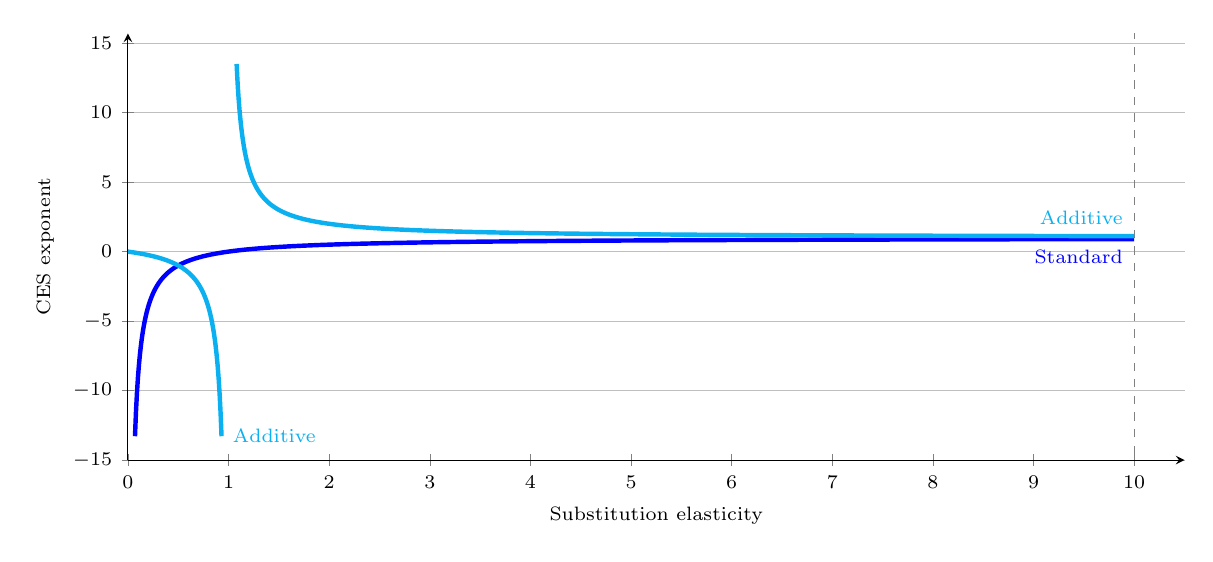
\begin{tikzpicture}
\begin{axis}[axis lines=left,xtick={0,1.0,...,10.0},xmin=0,xmax=10.5,
						     ytick={-15,-10,...,15},ymin=-15.0,ymax=15.7,
						     width=15cm,height=7cm,
x tick label style={
	/pgf/number format/.cd,
	fixed,
	fixed zerofill,
	precision=0,
	ymajorgrids,
	xlabel={\scriptsize{Substitution elasticity}},
	ylabel={\scriptsize{CES exponent}},
	/tikz/.cd
}]

\draw[dashed,color=gray] (10,-600) -- (10,600) ;

\addplot[mark=none,blue,ultra thick,domain=0.07:10,samples=1000]{(x-1)/x} node[below left] {\scriptsize{Standard}} ;
\addplot[mark=none,ProcessBlue,ultra thick,domain=0:0.93,samples=100]{x/(x-1)} node[right] {\scriptsize{Additive}} ;
\addplot[smooth,mark=none,ProcessBlue,ultra thick,domain=1.08:10,samples=1000]{x/(x-1)} node[above left] {\scriptsize{Additive}} ;

\end{axis}
\end{tikzpicture}
\end{figure}

\begin{figure}[h]
	\caption{\textbf{The CET exponent ($\nu$) as a function of the transformation elasticity}}
	\label{fig:CETFig}
	\centering

\pgfplotsset{every tick label/.append style={font=\scriptsize}}
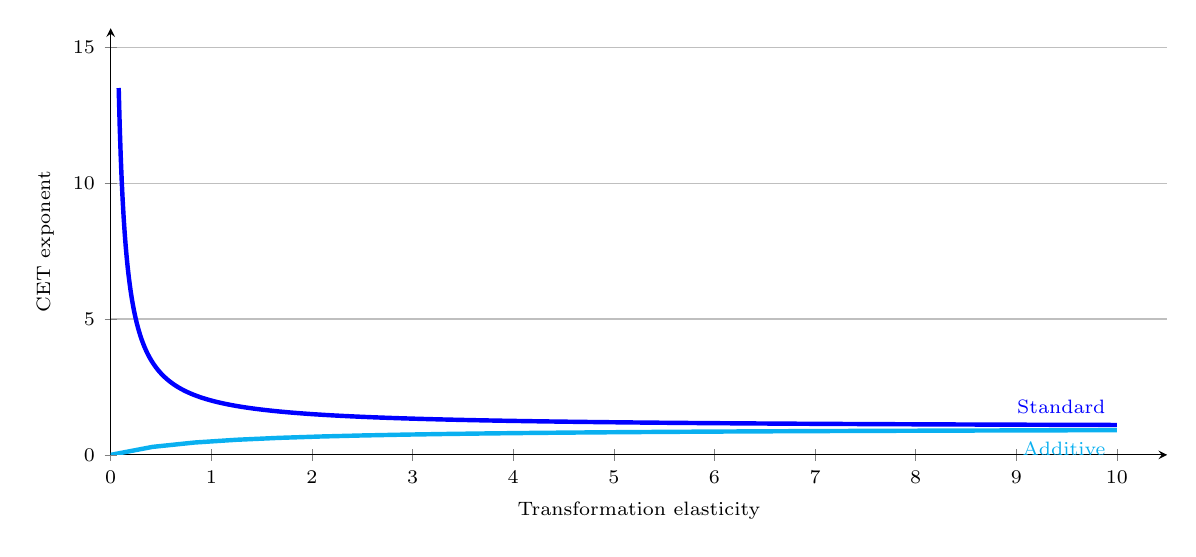
\begin{tikzpicture}[scale=1.0]
	\begin{axis}[axis lines=left,xtick={0,1.0,...,10.0},xmin=0,xmax=10.5,
ytick={0,5,...,15},ymin=0,ymax=15.7,
width=15cm,height=7cm,
x tick label style={
	/pgf/number format/.cd,
	fixed,
	fixed zerofill,
	precision=0,
	ymajorgrids,
	xlabel={\scriptsize{Transformation elasticity}},
	ylabel={\scriptsize{CET exponent}},
	/tikz/.cd
}]

\addplot[mark=none,blue,ultra thick,domain=0.08:10,samples=1000]{(x+1)/x} node[above left] {\scriptsize{Standard}} ;
\addplot[mark=none,ProcessBlue,ultra thick,domain=0:10]{x/(x+1)} node[below left] {\scriptsize{Additive}} ;

\end{axis}
\end{tikzpicture}
\end{figure}

\fi
